\documentclass[11pt]{article}
\pdfobjcompresslevel=0

\usepackage[review]{acl}

\usepackage{amsmath}
\usepackage{amssymb}
\usepackage{mathtools}
\usepackage{bm}
\usepackage{amsthm}

\usepackage{booktabs}
\usepackage{multirow}
\usepackage{array}
\usepackage{graphicx}
\usepackage{algorithm}
\usepackage{algpseudocode}
\usepackage{microtype}
\usepackage{enumitem}
\usepackage{xcolor}
\usepackage[nameinlink,capitalize]{cleveref}

% =========================================================
% Theorem environments
% =========================================================
\newtheorem{proposition}{Proposition}
\newtheorem{theorem}{Theorem}
\newtheorem{lemma}{Lemma}
\newtheorem{remark}{Remark}
\newtheorem{definition}{Definition}
\newtheorem{corollary}{Corollary}

% =========================================================
% CBG commands
% =========================================================
\newcommand{\R}{\mathbb{R}}
\newcommand{\Gh}{\mathcal{G}_{h}}
\newcommand{\Gb}{\mathcal{G}_{b}}
\newcommand{\Ghh}{\widehat{\mathcal{G}}_{h}}
\newcommand{\Gbh}{\widehat{\mathcal{G}}_{b}}
\newcommand{\Resc}{\rho_{\mathrm{esc}}}
\newcommand{\Barrier}{\mathcal{B}}
\newcommand{\U}{\mathcal{U}}
\newcommand{\Laln}{\mathcal{L}_{\mathrm{aln}}}
\newcommand{\Lbgn}{\mathcal{L}_{\mathrm{bgn}}}
\newcommand{\Lhfa}{\mathcal{L}_{\mathrm{hfa}}}
\newcommand{\rhohat}{\widehat{\rho}_{\mu}}
\newcommand{\rhoreg}{\rho_{\mu}}
\newcommand{\Lam}{\Lambda_{\theta}}
\newcommand{\Bmu}{\widehat{B}_{\mu}}
\newcommand{\Ft}{\widetilde{F}}
\newcommand{\Ch}{C_{h}}
\newcommand{\Cb}{C_{b}}
\newcommand{\etak}{\eta_{k}}
\newcommand{\Nb}{\mathcal{N}_{b}}
\newcommand{\Nh}{\mathcal{N}_{h}}
\newcommand{\diag}{\operatorname{diag}}
\newcommand{\row}{\operatorname{row}}
\newcommand{\tr}{\operatorname{tr}}
\newcommand{\Cth}{\widetilde{C}_{h}}
\newcommand{\Ctb}{\widetilde{C}_{b}}
\newcommand{\Pmu}{P_{\mu}}
\newcommand{\Smu}{S_{\mu}}

% Placeholder for results that do not exist yet. Never replace with a number
% that was not measured.
\newcommand{\tbd}{\textcolor{gray}{--}}
\newcommand{\todo}[1]{\textcolor{red}{[TODO: #1]}}


\title{\textbf{No Cheap Escape: Collateral Barrier Geometry for\\Self-Destructive Language Models}}
\author{Anonymous Authors}
\date{}

\begin{document}
\maketitle

\begin{abstract}
Safety alignment in open-weight language models can be removed by harmful fine-tuning or direct weight edits, often with little loss of capability. Self-destructive defenses make a particular harmful adaptation damage capability, but an adaptive attacker need not follow that direction and may find another that changes safety behavior at little benign cost. We propose the no-cheap-escape principle: a model should admit no admissible local parameter direction that causes a large safety-sensitive change at small benign cost. \textbf{Collateral Barrier Geometry (CBG)} instantiates this principle by comparing safety-sensitive and benign functional geometries and characterizing the weakest escape, the direction with the most safety change per unit of benign change, as a generalized eigenvalue problem. To make this trainable on minibatches, CBG damps the rank-deficient geometry with a rescaling-invariant metric and minimizes a normalized top-$k$ escape efficiency, computed exactly from a small Gram matrix of per-example gradients and differentiated at the cost of two additional gradient evaluations. The theory is local; we evaluate CBG empirically under standard, parameter-efficient and adaptive low-collateral fine-tuning attacks and under refusal-direction orthogonalization.
\end{abstract}



\section{Introduction}
\label{sec:introduction}

Safety alignment reduces harmful behavior in large language models (LLMs), but it often does not survive modification after release. Fine-tuning on a few harmful examples can remove refusal behavior while leaving general capability largely intact~\citep{qi2024finetuning}, and a direct weight edit can remove a single refusal direction~\citep{arditi2024refusal}. For open-weight models, alignment must therefore concern not only the released checkpoint but also how its behavior responds to subsequent parameter changes.

Many defenses try to make harmful fine-tuning harder~\citep{huang2024vaccine,huang2025booster,rosati2024repnoise,tamirisa2025tar}, yet several lose their protection under stronger attacks~\citep{qi2025evaluating}. Self-destructive alignment takes a complementary route~\citep{henderson2023self}: rather than only resisting harmful adaptation, it makes that adaptation damage benign capability. The closest prior work, SEAM~\citep{wang2026seam}, trains the model so that the gradient of a harmful loss opposes the gradient of a benign loss, so following the former degrades the latter.

Such coupling makes one harmful optimization direction destructive. It does not establish that every other way of changing safety behavior is also expensive. An adaptive attacker is not bound to the defender's harmful loss: it may change the objective, optimizer or trainable parameters, add a regularizer that preserves benign behavior, or edit weights directly. SEAM's own analysis leaves capability-preserving attacks as an open question and reports that refusal-direction orthogonalization remains effective against SEAM-defended models. This raises a sharper question: \emph{what is the cheapest way to change safety-sensitive behavior while preserving benign functionality?}

We make this question the defense target through the \emph{no-cheap-escape principle}: a self-destructive model should admit no admissible local parameter direction that produces a large safety-sensitive change at small benign cost. The principle shifts attention from one harmful trajectory to the direction most favorable to the attacker. If even that direction is expensive, no cheap local alternative exists; if it is not, protecting other directions matters little.

We instantiate the principle as \textbf{Collateral Barrier Geometry (CBG)}. For every admissible update direction, CBG compares how much the update moves the model's preference between safe and harmful responses with how much it moves behavior on benign inputs. The direction with the largest safety change per unit of benign change is the \emph{weakest escape}; its efficiency is a generalized eigenvalue of the two geometries and is inversely proportional to a \emph{collateral barrier}, the minimum modeled benign cost of a prescribed safety-sensitive change (\cref{fig:cbg-overview}). CBG trains the model to suppress its leading escapes. Doing so on minibatches requires a damped, rescaling-aware and normalized form of the efficiency, which we derive in \cref{sec:method} and which can be computed exactly and differentiated at the cost of two additional gradient evaluations per step.

\begin{figure*}[t]
    \centering
    \includegraphics[width=\textwidth]{CBG_method.pdf}
    \caption{CBG searches for low-collateral safety-changing directions and reshapes the local geometry so that leading escapes incur greater benign collateral.}
    \label{fig:cbg-overview}
\end{figure*}

The theory characterizes a local geometry and does not guarantee robustness to long fine-tuning trajectories or non-local weight edits; we test those settings empirically. Our contributions are:
\begin{itemize}[leftmargin=*]
\item We introduce the no-cheap-escape principle and formulate self-destructive alignment as a worst-direction benign-collateral problem, characterized spectrally by a collateral barrier.
\item We develop CBG, a trainable objective that remains well posed on minibatches, with an exact Gram-based spectral solver and an efficient gradient estimator.
\item We evaluate CBG under standard, parameter-efficient and adaptive low-collateral fine-tuning attacks and under orthogonalization, and analyze whether the learned geometry predicts attack outcomes.
\end{itemize}





\section{Related Work}
\label{sec:related}

\paragraph{Harmful fine-tuning and defenses.}
Safety alignment can be removed after release by fine-tuning~\citep{qi2024finetuning} or by deleting a refusal direction~\citep{arditi2024refusal}; it is concentrated in the first output tokens~\citep{qi2025safety} and holds only within a local basin of the weights~\citep{peng2024navigating}. Existing defenses each target a specific perturbation model: representation drift~\citep{huang2024vaccine,liu2024targeted}, harmful-representation suppression~\citep{rosati2024repnoise}, simulated or meta-learned attacks~\citep{huang2025booster,tamirisa2025tar}, constrained user fine-tuning~\citep{huang2024lisa,li2025salora}, and non-fine-tunable learning~\citep{deng2024sophon}. Such protection often fails when the attacker changes the learning rate, optimizer, data or objective~\citep{qi2025evaluating,zloczower2026one}.

\paragraph{Self-destructive alignment.}
Self-destructive methods instead make safety removal degrade benign capability~\citep{henderson2023self}, by degrading harmful answers~\citep{chen2025sdd}, embedding a collapse trap~\citep{yi2026ctrap}, or targeting harmful RL fine-tuning~\citep{feng2026tokenbuncher}. Closest to our work, SEAM~\citep{wang2026seam} anti-aligns the mean harmful and benign gradients and amplifies the effect with gradient ascent on harmful data. SEAM shapes the relation between two gradient directions of harmful adaptation; CBG instead penalizes the most collateral-efficient safety-changing directions over an admissible update space, regardless of their sign or loss. In a limiting case CBG reduces to a multi-direction analogue of SEAM's coupling (\cref{rem:seam}), and the two can be combined.

\paragraph{Geometric tools.}
CBG builds on established tools: Fisher geometry~\citep{amari1998natural,martens2020new,kunstner2019limitations}, generalized eigenproblems and sums of top eigenvalues~\citep{parlett1998symmetric,golub2013matrix,overton1993optimality}, and scale-invariant sharpness~\citep{dinh2017sharp,foret2021sharpness,kwon2021asam}; HarmAlign also applies spectral analysis to safety~\citep{rosati2026harmalign}. Our contribution is not these tools but the formulation of self-destructive alignment as a worst-direction collateral problem and an objective that keeps it trainable on minibatches.



\section{Preliminaries}
\label{sec:preliminaries}

\paragraph{Threat model.}
A defender releases a safety-aligned model $f_\theta$, obtained by further training an aligned model $f_{\theta_0}$. A white-box adversary with harmful data $\mathcal D_{\mathrm{atk}}=\{(x_l,y_l^h)\}_{l=1}^{N}$ attempts to remove safety behavior. Starting from $\theta$, a standard attack minimizes
\begin{equation}
\Lhfa(\theta')=\mathbb E_{(x,y^h)\sim\mathcal D_{\mathrm{atk}}}\,\ell\bigl(f_{\theta'}(x),y^h\bigr)
\label{eq:hfa}
\end{equation}
over $\theta'$, where $\ell$ is the token-level cross-entropy. Adaptive adversaries may change the objective (e.g., by adding a penalty that preserves benign behavior), the optimizer, the learning rate, the trainable parameters or the parameterization (full fine-tuning or LoRA), or may edit weights directly. The adversary succeeds if the modified model is both harmful and still useful.

\paragraph{Admissible local updates.}
We write an attack-induced change as $u=\theta'-\theta$ and do not assume that it follows the harmful gradient. Let $\U\subseteq\R^p$ be a linear subspace of admissible directions; by default $\U$ spans the weight matrices of all linear layers in the transformer blocks and excludes embeddings, normalization gains and the output head. The set $\mathcal V$ of updates a particular attacker can realize need not be a subspace: full fine-tuning of these matrices gives $\mathcal V=\U$, whereas rank-$r$ LoRA gives the matrices of rank at most $r$. Whenever $\mathcal V\subseteq\U$, the barrier defined in \cref{sec:formulation} is at least as large over $\mathcal V$ as over $\U$ (\cref{prop:monotone}), so it suffices to analyze $\U$. Updates with components outside $\U$ are not covered by this argument and are evaluated empirically. A direction in $\U$ that substantially changes safety-sensitive behavior at little benign functional cost is a \emph{low-collateral escape}.



\section{Methodology}
\label{sec:method}

CBG asks how cheaply, in benign functional terms, an admissible parameter change can move safety-sensitive behavior. We define this cost (\cref{sec:formulation}), make it well posed on minibatches (\cref{sec:practical}), and optimize it at LLM scale (\cref{sec:objective}).

% ---------------------------------------------------------
\subsection{Escape Geometry}
\label{sec:formulation}

\paragraph{Measurements.}
Safety data $\mathcal D_h=\{(x_i,y_i^s,y_i^h)\}_{i=1}^{m}$ pair each prompt with a safe and a harmful response; benign data $\mathcal D_b=\{(x_j,y_j)\}_{j=1}^{n}$ contain ordinary instructions. Each safety example contributes a token-normalized preference margin
\begin{equation}
\begin{aligned}
h_i(\theta)={}&\tfrac{1}{|y_i^h|}\log p_\theta(y_i^h\mid x_i)\\
&-\tfrac{1}{|y_i^s|}\log p_\theta(y_i^s\mid x_i),
\end{aligned}
\label{eq:safety_margin}
\end{equation}
which increases as the model moves toward the harmful response. Each benign example contributes the log-likelihood of tokens sampled from the model itself: under teacher forcing on $y_j$ we draw $\hat y_{j,t}\sim p_\theta(\cdot\mid x_j,y_{j,<t})$, fix the samples within a step, and set
\begin{equation}
F_{b,j}(\vartheta)=\textstyle\sum_{t}\log p_\vartheta(\hat y_{j,t}\mid x_j,y_{j,<t}).
\label{eq:mc_fisher}
\end{equation}
With $F_h=(h_i)_{i\le m}$, the $m+n$ weighted measurements $\Ft=(F_h/\sqrt m;\,F_b/\sqrt n)$ are indexed by $e$, and their Jacobian restricted to $\U$ is $C=[\Ch;\Cb]$ with rows $c_e$. For $u\in\U$,
\begin{equation}
Q_h(u)=\|\Ch u\|_2^2,\qquad Q_b(u)=\|\Cb u\|_2^2
\label{eq:metrics}
\end{equation}
are the first-order \emph{safety-sensitive displacement} and \emph{benign collateral} of $u$. $Q_h$ is sign-agnostic: it measures how strongly $u$ moves safety preferences, not in which direction. Because targets are sampled, $\mathbb E_{\hat y}[Q_b(u)]$ is the token-summed Fisher form, i.e.\ twice the second-order benign KL divergence between the current and the modified model (\cref{prop:mcfisher}). $Q_b$ therefore charges any change of the benign predictive distribution, which observed targets would not~\citep{kunstner2019limitations}.

\paragraph{Weakest escape and barrier.}
The attacker's most favorable local option is the direction with the largest displacement per unit of collateral.
\begin{definition}
\label{def:escape}
The \emph{escape efficiency} and the \emph{collateral barrier} at displacement $\gamma>0$ are
\begin{equation}
\begin{gathered}
\Resc=\sup_{u\in\U:\,Q_h(u)>0}\frac{Q_h(u)}{Q_b(u)},\\
\Barrier_\gamma=\inf_{u\in\U}\bigl\{\tfrac12Q_b(u):Q_h(u)\ge\gamma^2\bigr\},
\end{gathered}
\label{eq:rho_esc}
\end{equation}
with $c/0=+\infty$ for $c>0$ and $\sup\emptyset=0$. A maximizer is a \emph{weakest escape}.
\end{definition}
With the conventions $1/0=+\infty$ and $1/{+\infty}=0$,
\begin{equation}
\Barrier_\gamma=\frac{\gamma^2}{2\Resc}
\label{eq:barrier_identity}
\end{equation}
in every case, and $\Resc$ is finite, equal to the largest generalized eigenvalue of $(\Ch^\top\Ch,\Cb^\top\Cb)$ on the benign support of $\U$, exactly when $\U\cap\ker\Cb\subseteq\U\cap\ker\Ch$ (\cref{thm:barrier}). This is a standard generalized eigenproblem; it motivates the objective and is not a main result.

\paragraph{Finite-sample degeneracy.}
On a minibatch, $\operatorname{rank}\Cb\le n\ll\dim\U$, and the kernel condition holds only if every safety-margin gradient lies in the span of the $n$ benign gradients (\cref{prop:degenerate}). Generically it fails, so $\Resc=+\infty$ and $\Barrier_\gamma=0$: the benign sample leaves most directions unobserved, and the undamped objective reports a free escape through them.



\subsection{Trainable Geometry}
\label{sec:practical}

\paragraph{Relative coordinates.}
Unobserved directions need a movement cost, but transformers admit exact function-preserving diagonal rescalings (e.g., an MLP up-projection row against the matching down-projection column), and a Euclidean cost can be lowered by them without any change in behavior (\cref{prop:reparam}). Following adaptive sharpness~\citep{kwon2021asam}, we measure updates in relative units,
\begin{equation}
u=D_\theta\delta,\qquad D_\theta=\diag(\theta\odot\theta+\xi^2)^{1/2},
\label{eq:relative}
\end{equation}
so that $\|\delta\|_2^2=u^\top\Lam u$ with $\Lam=D_\theta^{-2}$. The relative Jacobian is $\widetilde C=CD_\theta=[\Cth;\Ctb]$, and its Gram $K=\widetilde C\widetilde C^\top=C\Lam^{-1}C^\top$, with blocks $K_{hh},K_{hb},K_{bb}$, is $(m+n)\times(m+n)$. For $\xi=0$ every quantity below is invariant under diagonal rescalings that preserve $F_h$ and $F_b$; the floor $\xi>0$ makes this approximate for $|\theta_i|\lesssim\xi$, and symmetries that mix coordinates are not covered.

\paragraph{Damping as soft projection.}
We charge movement $\mu\|\delta\|^2$ in addition to collateral. The damped efficiency is
\begin{equation}
\begin{aligned}
\rhoreg&=\max_{\delta\ne0}\frac{\|\Cth\delta\|^2}{\|\Ctb\delta\|^2+\mu\|\delta\|^2}
=\frac{\lambda_{\max}\bigl(\Cth\Pmu\Cth^{\top}\bigr)}{\mu},\\
\Pmu&=\mu\bigl(\Ctb^{\top}\Ctb+\mu I\bigr)^{-1},
\end{aligned}
\label{eq:damped}
\end{equation}
and the damped barrier $\Barrier^{(\mu)}_\gamma$, the least total cost $\tfrac12\bigl(Q_b(u)+\mu\,u^\top\Lam u\bigr)$ over $u\in\U$ with $Q_h(u)\ge\gamma^2$, equals $\gamma^2/(2\rhoreg)$ without any kernel condition; moreover $\rhoreg\uparrow\Resc$ as $\mu\downarrow0$ (\cref{prop:damped}). The matrix $0\preceq\Pmu\preceq I$ is a \emph{soft projector}: a direction with benign sensitivity $s^2$ is shrunk by $\mu/(s^2+\mu)$, and an unobserved direction passes unchanged. By the push-through identity, the projected safety Gram is a Schur complement of $K$,
\begin{equation}
\begin{aligned}
\Cth\Pmu\Cth^{\top}=\Smu:={}&K_{hh}\\
&-K_{hb}(\mu I_n+K_{bb})^{-1}K_{hb}^\top ,
\end{aligned}
\label{eq:reduced}
\end{equation}
i.e.\ the safety Gram with the part explained by benign sensitivity removed. We set $\mu=\kappa_\mu\tr(K_{bb})/n$, a multiple of the mean eigenvalue of the benign Gram, so $\kappa_\mu$ fixes the sensitivity below which a benign direction counts as unobserved.

\paragraph{Normalized top-$k$ efficiency.}
Minimizing $\rhoreg$ leaves two loopholes. \emph{Safety flattening}: $\rhoreg$ scales with $\|\Cth\|^2$, so shrinking safety sensitivity lowers it without making any escape costlier. \emph{Mode substitution}: suppressing only the leading escape lets the next one dominate. We therefore train the fraction of the top-$k$ relative safety sensitivity that survives the soft projection,
\begin{equation}
\begin{gathered}
\etak(\theta)=\frac{\sigma_{1:k}}{\nu_{1:k}}\in(0,1],\\
\sigma_j=\lambda_j(\Smu),\qquad \nu_j=\lambda_j(K_{hh}),
\end{gathered}
\label{eq:eta}
\end{equation}
where $\sigma_{1:k}=\sum_{j\le k}\sigma_j$, likewise $\nu_{1:k}$, and $k\le\operatorname{rank}\Cth\le m$. It is at most one because $\Smu\preceq K_{hh}$, and it needs only two $m\times m$ eigenproblems. It is unchanged by uniform safety flattening ($\Cth\mapsto t\Cth$) and by uniform benign inflation ($\Ctb\mapsto t\Ctb$, since $\mu$ scales with $K_{bb}$). For $k=1$, $1/\eta_1$ is the factor by which benign collateral raises the cost of the cheapest local escape over a movement-only cost (\cref{prop:eta}); as $\mu\downarrow0$, $\eta_1$ tends to a squared sine between the safety and benign gradient spans, a multi-direction, sign-agnostic analogue of SEAM's gradient coupling (\cref{rem:seam}).

The escapes follow from the same Gram. For $\Smu\phi_j=\sigma_j\phi_j$ with $\|\phi_j\|=1$, let
\begin{equation}
\begin{gathered}
z_j=(\mu I_n+K_{bb})^{-1}K_{hb}^\top\phi_j,\\
\psi_j=(\phi_j;\,-z_j)\in\R^{m+n}.
\end{gathered}
\label{eq:escape}
\end{equation}
Then $u_j=D_\theta\widetilde C^\top\psi_j/\sqrt{\mu\sigma_j}$ is the $j$-th weakest damped escape, with efficiency $\rho_j=\sigma_j/\mu$ and unit total cost (\cref{prop:reduced}).



\subsection{Objective and Optimization}
\label{sec:objective}

\paragraph{Objective.}
The defense minimizes
\begin{equation}
\widehat{\mathcal L}_{\mathrm{train}}=\Laln+\alpha\Lbgn+\beta\log\etak ,
\label{eq:training_objective}
\end{equation}
where $\Laln$ is the supervised loss of $y_i^s$ given $x_i$ and $\Lbgn$ is the token-level $\mathrm{KL}(p_{\theta_0}\Vert p_\theta)$ from the aligned model on benign data. The gradient flows through $\mu$: $\etak$ is invariant to benign inflation only because $\mu$ moves with $K_{bb}$, and detaching $\mu$ would reward inflating benign sensitivity (\cref{rem:mu}). The objective targets the collateral incurred per unit of safety change, not the amount of safety change an attack must achieve; it is therefore complementary to terms that increase the latter, such as SEAM's unlearning loss (\cref{prop:path}), and we evaluate the combination as CBG+UL. Minibatch spectral estimates are biased (\cref{prop:jensen}), so we use many short benign sequences ($n\ge4m$). The objective shapes local geometry; it is not a global robustness guarantee.

\paragraph{Gradient through the Gram.}
The objective depends on $\theta$ only through $K$, so its gradient is the pull-back of one small matrix. Let $K_{hh}\phi'_j=\nu_j\phi'_j$ with $\|\phi'_j\|=1$, $\psi'_j=(\phi'_j;\,0)$ and $E_b=0_m\oplus I_n$. At a spectral gap ($\sigma_k>\sigma_{k+1}$, $\nu_k>\nu_{k+1}$), $G=\partial\log\etak/\partial K$ is
\begin{equation}
\begin{aligned}
G={}&\frac{1}{\sigma_{1:k}}\textstyle\sum_{j\le k}\bigl(\psi_j\psi_j^\top+\tfrac{\kappa_\mu}{n}\|z_j\|^2E_b\bigr)\\
&-\frac{1}{\nu_{1:k}}\textstyle\sum_{j\le k}\psi'_j\psi_j'^\top
\end{aligned}
\label{eq:G}
\end{equation}
(\cref{prop:gradient}), where the $E_b$ term is the entire effect of differentiating $\mu$. Pulling $G$ back through $K=C\Lam^{-1}C^\top$ gives
\begin{equation}
\begin{gathered}
\nabla_\theta\log\etak=2\textstyle\sum_{e}H_{\Ft_e}w_e+d_\Lambda,\\
w_e=\Lam^{-1}C^\top G\mathbf 1_e,\quad d_\Lambda=2\,\theta\odot\operatorname{diag}(C^\top GC)
\end{gathered}
\label{eq:gram_grad}
\end{equation}
(\cref{prop:gram}), where $H_{\Ft_e}$ is the Hessian of the $e$-th measurement and $d_\Lambda$ comes from the dependence of $\Lam$ on $\theta$. Without a gap, the same expressions are Clarke subgradients of the two spectral sums.

\paragraph{Curvature term.}
The first term of \cref{eq:gram_grad} is a sum of $m+n$ Hessian--vector products with different directions. We obtain it from ordinary gradients by a centered difference along one shared direction. For any random pair $a,b\in\R^{m+n}$ with $\mathbb E[ab^\top]=G$, set $\Omega=a^\top\Ft$ and $w=\Lam^{-1}C^\top b$. Then
\begin{equation}
\begin{aligned}
\nabla_\theta\log\etak={}&\mathbb E_{a,b}\Bigl[\tfrac{1}{\varepsilon}\bigl(\nabla\Omega(\theta+\varepsilon w)\\
&-\nabla\Omega(\theta-\varepsilon w)\bigr)\Bigr]+d_\Lambda+\mathcal O(\varepsilon^2)
\end{aligned}
\label{eq:outer}
\end{equation}
(\cref{prop:randomized}). We draw $a=V|\Gamma|^{1/2}s$ and $b=V\operatorname{sgn}(\Gamma)|\Gamma|^{1/2}s$ from the eigendecomposition $G=V\Gamma V^\top$ and Rademacher signs $s$. The estimate is unbiased up to $\mathcal O(\varepsilon^2)$ but has sign-draw variance; draws can be averaged at two passes each. A deterministic alternative perturbs each example $e$ along its own $w_e$, which removes this variance at a higher cost per pass (\cref{app:impl}); \cref{sec:ablation} compares the two.

\paragraph{Algorithm.}
\Cref{alg:cbg} lists one step. The two perturbed passes reuse the minibatch, the samples $\hat y$ and the signs, and their average also yields the base-loss gradient up to $\mathcal O(\varepsilon^2)$. The step $\varepsilon$ sets the root-mean-square relative perturbation $\|\Lam^{1/2}\varepsilon w\|/\sqrt{\dim\U}$ to a radius $r$, read off the Gram through $\|\Lam^{1/2}w\|^2=b^\top Kb$. The perturbation is applied to fp32 master weights~\citep{micikevicius2018mixed}, and $r$ is chosen against an exact Hessian--vector product on a small model so that the compute precision resolves it (\cref{app:impl}).

\begin{algorithm}[t]
\caption{One CBG training step}
\label{alg:cbg}
\small
\begin{algorithmic}[1]
\Require weights $\theta$ (fp32); safety batch $(x_i,y_i^s,y_i^h)_{i\le m}$; benign batch $(x_j,y_j)_{j\le n}$; $\alpha,\beta,\kappa_\mu,k,\xi,r$
\State Forward at $\theta$; sample $\hat y$ from benign logits; form $\Ft$; store layer inputs $X$
\State Backward of $\mathbf 1^\top\Ft$; store output gradients $\Delta$; accumulate $K$ from $(X,\Delta)$
\State $\mu\gets\kappa_\mu\tr(K_{bb})/n$; top-$k$ eigenpairs of $\Smu$ and $K_{hh}$; $\etak$ and $G$ (\cref{eq:reduced,eq:eta,eq:G})
\State Draw $s$; form $a,b$; one chunked pass over $(X,\Delta)$ gives $w=\Lam^{-1}C^\top b$ and $d_\Lambda$
\State $\varepsilon\gets r\sqrt{\dim\U/(b^\top Kb)}$;\ $g\gets0$
\For{$\tau\in\{+1,-1\}$}
  \State Forward at $\theta+\tau\varepsilon w$ with the same $\hat y$
  \State $g\mathrel{+}=\nabla\bigl[\tau\tfrac{\beta}{\varepsilon}\,a^\top\Ft+\tfrac12(\Laln+\alpha\Lbgn)\bigr]$
\EndFor
\State $\theta\gets\textsc{OptimizerStep}(\theta,\ g+\beta d_\Lambda)$
\end{algorithmic}
\end{algorithm}



\providecommand{\tbd}{--}

\section{Experiments}
\label{sec:experiments}

We report the experiments in the order in which they were run. CBG was configured on a validation protocol (\cref{sec:exp_selection}) and then compared with SEAM, SDD and CTRAP under one shared evaluation protocol (\cref{sec:exp_main}). We then analyze how CBG changes the geometry it targets (\cref{sec:barrier_analysis}). The remaining experiments compare CBG with the undefended Base model only. In all tables, gray dashes (\tbd) mark planned measurements not made yet, and black dashes mark entries that do not apply or were not measured for that configuration.



\subsection{Experimental Setting}
\label{sec:setting}

\paragraph{Models.}
All defenses start from Llama-2-7B-Chat (\texttt{meta-llama/Llama-2-7b-chat-hf}, revision \texttt{f5db02db}). The same checkpoint is the frozen reference $\theta_0$ of $\Lbgn$ and the \emph{Base} model of every table.

\paragraph{Data.}
We follow SEAM's data recipe~\citep{wang2026seam}. The BeaverTails~\citep{ji2023beavertails} rows of the public RepNoise release that are unsafe and have a refusal are shuffled with seed 42 and split into row-disjoint pools:
\begin{itemize}
  \item \textbf{Defense set $\mathcal D_h$}: rows 1--4{,}000, safety pairs $(x, y^h, y^s)$ with harmful responses $y^h$ and refusals $y^s$.
  \item \textbf{Benign set $\mathcal D_b$}: the first 4{,}000 Alpaca-cleaned samples~\citep{taori2023alpaca} after a seed-42 shuffle.
  \item \textbf{Harmful attack set}: rows 4{,}001--5{,}000.
  \item \textbf{Harmfulness test set}: the first 100 BeaverTails \texttt{30k\_test} prompts, in file order, that pass the category filter of SEAM's evaluation script.
  \item \textbf{Validation split} (CBG only, \cref{sec:exp_selection}): 1{,}000 further rows (from row 5{,}001 on, completed from BeaverTails \texttt{330k\_train}), prompt-disjoint from all of the above; 900 form the validation attack and 100 the validation prompts.
  \item \textbf{Geometry set $\mathcal D_{\mathrm{geo}}$}: 8 fixed batches of $m=8$ pairs and $n=32$ Alpaca rows (64 pairs prompt-disjoint from the pools above; Alpaca rows 4{,}001--4{,}256 of the same shuffle).
\end{itemize}
The defense, attack and test pools are disjoint as rows but not as prompts, because BeaverTails repeats prompts across rows and splits. As in SEAM's evaluator we do not remove repeats: in the main runs, 548 to 623 of the 1{,}000 attack rows share their prompt with a row of a defense set used in the same run, up to 56 of the 100 test prompts do, and 304 attack rows have a prompt that also occurs in BeaverTails \texttt{30k\_test}. Benign fine-tuning data (\cref{sec:exp_main}) are 1{,}000 Alpaca-cleaned rows drawn after the first 4{,}000 of the shuffle, so they are disjoint from $\mathcal D_b$. Training texts use SEAM's format \texttt{Question: \{prompt\}\textbackslash nAnswer: \{response\}} and are truncated to 256 tokens.

\paragraph{CBG.}
\begin{itemize}
  \item \textbf{Measured set and batch:} $\U$ is the weight of every linear layer inside the transformer blocks (embeddings, norms and the output head are excluded). Each CBG step uses $m=8$ safety pairs and $n=32$ benign sequences, each at most 256 tokens.
  \item \textbf{Geometry hyperparameters:} $k=4$, $\kappa_\mu=1$, $\xi=10^{-3}$, $\alpha=1$, $\beta=0.1$ (\cref{sec:exp_selection}).
  \item \textbf{Curvature term:} an exact Hessian--vector product in TF32, with one shared sign draw. Before training we check it against an FP32 Hessian--vector product and a central finite difference.
  \item \textbf{Two-point geometry:} the geometry term is the mean of $\log\etak$ at $\theta$ and at $\theta'=\theta-10^{-5}\operatorname{sign}(\nabla\mathcal L_{\mathrm{harm}}(\theta))$, where $\mathcal L_{\mathrm{harm}}$ is the cross-entropy of $y^h$ on the current safety batch. The step $10^{-5}$ was calibrated on Base against a real attack (\cref{sec:exp_selection}).
  \item \textbf{Gradient balancing:} on each tensor, the geometry gradient is rescaled to the norm of the gradient of $\Laln+\alpha\Lbgn$ on that tensor, so $\beta$ sets only its direction. A geometry gradient above three times the median of the last 16 is clipped.
  \item \textbf{Lazy geometry:} the full CBG step runs every 4 optimizer steps, and its geometry gradient is reused on the three intermediate steps.
  \item \textbf{Optimization:} full-parameter AdamW, learning rate $2\times10^{-5}$, cosine schedule with 10\% warmup, no weight decay or clipping, 500 steps, model split by layer over two H200 GPUs.
  \item \textbf{Utility gate:} training stops if the mean $\Lbgn$ of the last 20 steps exceeds $0.3$ at step 100 or 250. The selected run passed both checks (0.175 and 0.286).
\end{itemize}
Two-point geometry, gradient balancing and lazy reuse change how the objective of \cref{sec:objective} is optimized, not the geometry it measures.

\paragraph{Baselines.}
In the main comparison (\cref{sec:exp_main}) we compare against three defenses, each trained from the same Llama-2-7B-Chat checkpoint:
\begin{itemize}
  \item \textbf{SEAM}~\citep{wang2026seam}: its released training code and default configuration, 500 steps at batch 8 in FP32, on the 4{,}000 defense rows above. In this code version the safety losses skip the first response token because of an off-by-one mask; we keep it, so the baseline is the released implementation.
  \item \textbf{SDD}~\citep{chen2025sdd}: no training code is released, so we reimplement it from the paper. It fine-tunes on 8{,}000 harmful prompts paired with irrelevant Alpaca answers (cosine similarity $\le0.25$), for 500 steps at learning rate $5\times10^{-7}$; the paper also draws answers from LIMA.
  \item \textbf{CTRAP}~\citep{yi2025ctrap}: its released trainer with LoRA (rank 32 on the query, key and value projections), merged after 500 steps.
\end{itemize}
SDD and CTRAP use their own prompt templates in training, whereas the evaluation uses SEAM's template for every model. This may favor SEAM and CBG, which are trained with it. All other experiments compare CBG with the undefended Base model only.

\paragraph{Attack protocol.}
Every attack starts from the clean (un-attacked) checkpoint of the evaluated model; attacks are never chained. Unless stated otherwise, an attack is:
\begin{itemize}
  \item full-parameter supervised fine-tuning for 250 steps on 1{,}000 samples, effective batch size 4 (one sample with four accumulation steps);
  \item AdamW (PyTorch implementation) on BF16 weights, cosine schedule, 10\% warmup, weight decay $0.01$, no gradient clipping, gradient checkpointing, seed 42, one H100 (80\,GB) per attack.
\end{itemize}
As in SEAM's evaluation script, each training text is padded to 256 tokens with the end-of-sequence token, and the labels equal the input ids, padding included. The attack loss therefore includes padding tokens.

\paragraph{Metrics.}
\begin{itemize}
  \item \textbf{Harmfulness score (HS):} the mean probability of the \texttt{harmful} label assigned by the BeaverTails DeBERTa classifier\footnote{\texttt{domenicrosati/deberta-v3-xsmall-beavertails-harmful-qa-classifier}.} to prompt plus response, truncated to 512 tokens. An empty response scores 0. Responses are generated with at most 50 new tokens by seeded sampling (temperature $0.6$, top-$p$ $0.9$), the Llama-2-Chat generation defaults on which SEAM's evaluation script relies. We also report the fraction of responses with score $>0.5$.
  \item \textbf{Zero-shot score (ZS):} the mean zero-shot accuracy (\texttt{acc}) on TruthfulQA (MC1), MMLU, HellaSwag and ARC-Easy, using LM Evaluation Harness~\citep{gao2024harness} 0.4.7.
  \item \textbf{Compromised:} as in SEAM, an attacked model is \emph{compromised} if HS $>10\%$ while ZS $>30\%$. Low HS together with low ZS is \emph{self-destruction}. Low HS with intact ZS and a high attack loss is a failed attack, not a defense, so we report the attack's training loss with every attacked row.
  \item \textbf{Geometry:} we report $\etak$ together with $\sigma_{1:k}$, $\nu_{1:k}$, $\tr K_{bb}$ and the effective ranks of $K_{hh}$ and $K_{bb}$, all averaged over the 8 batches of $\mathcal D_{\mathrm{geo}}$ ($\mu=\kappa_\mu\tr K_{bb}/n$, $m=8$, $n=32$). The minibatch $\Resc$ and $\Barrier_\gamma$ are not reported, since they are $+\infty$ and $0$ by construction (\cref{prop:degenerate}).
\end{itemize}



\subsection{Hyperparameter Selection}
\label{sec:exp_selection}

\paragraph{Validation protocol.}
CBG was configured without the test split, with two criteria:
\begin{itemize}
  \item the change of the held-out $\log\etak$ on $\mathcal D_{\mathrm{geo}}$ during training, together with the benign drift $\Lbgn$;
  \item one harmful attack on the validation split (900 rows, 225 steps, learning rate $10^{-4}$), with HS from greedy decoding on the 100 validation prompts and ARC-Easy accuracy.
\end{itemize}
These validation attacks ran on one L40S (48\,GB), so they use paged 8-bit AdamW; their numbers are comparable with each other but not with \cref{tab:main}. For three configurations we also measured $\log\etak$ after the first 25 steps of the validation attack. This tests whether the change in geometry outlasts the start of an attack.

\paragraph{Configurations.}
\Cref{tab:selection} lists every configuration we trained.
\begin{itemize}
  \item \textbf{Global geometry} (no balancing; $\beta=0.01$ and $\beta=0.1$): with $\beta=0.1$, $\log\etak$ fell by $1.36$, but benign drift grew ($\Lbgn\approx0.55$) and pre-attack ZS fell to 41.1.
  \item \textbf{Per-tensor cap and balancing (pilots A and B)}: these keep $\Lbgn$ small. After 25 attack steps, however, pilot B's held-out $\log\etak$ had returned from $-0.60$ to $-0.11$ (Base: $-0.05$), so the barrier is local.
  \item \textbf{Two-point geometry} (pilot C, step $5\times10^{-4}$): this step raised $\mathcal L_{\mathrm{harm}}(\theta')$ from 1.94 to 6.09, so $\theta'$ lay where the harmful loss rises again, not where an attack goes. The run was stopped after 4 steps, and we calibrated the step on Base against a real attack:
    \begin{itemize}
      \item $\mathcal L_{\mathrm{harm}}$ is 1.96 at $\theta$ and 1.68 after 25 attack steps at $10^{-4}$;
      \item one sign step lowers it to 1.26 at $10^{-5}$ and 1.03 at $3\times10^{-5}$, but raises it again at larger steps (3.29 at $3\times10^{-4}$).
    \end{itemize}
    We used $10^{-5}$, which moves $\mathcal L_{\mathrm{harm}}$ about as far as the early attack does while staying in the decreasing range. With this step (pilot C2), $\log\etak$ fell by $1.09$ in 100 steps and stayed at $-0.39$ after 25 attack steps.
  \item \textbf{CBG+UL} (SEAM's unlearning loss added): the geometry barely changed ($|\Delta\log\etak|\le0.10$ after 100 steps).
\end{itemize}

\paragraph{Outcome.}
No configuration lowered the validation HS below Base: pilot B reached 57.1 and C2 60.8, against 56.8 for Base, with the same attack loss. We selected C2 because it produced the largest and most persistent geometry change within the utility gate, and trained it for 500 steps (\emph{CBG} below).

Two early configurations, global $\beta=0.01$ and CBG+UL, were also attacked on the test split before this protocol was fixed. They are marked $^\ast$ in \cref{tab:selection} and did not reduce HS either.

\begin{table*}[t]
\centering
\small
\caption{CBG configurations tried. $\Delta\log\etak$: change of the held-out $\log\etak$ on $\mathcal D_{\mathrm{geo}}$ from step 0 ($-0.024$) to step 100 and to the end of training. ``After atk.'': held-out $\log\etak$ after 25 steps of the validation attack at $10^{-4}$. $\Lbgn$: mean over the last 20 training steps. Val.\ HS / ARC: validation attack at $10^{-4}$ (L40S protocol, greedy). $^\dagger$validation attack at $5\times10^{-5}$. $^\ast$evaluated on the test split during exploration (L40S protocol, greedy): pre-attack HS / ZS, and HS / ZS after an attack at $5\times10^{-5}$.}
\label{tab:selection}
\resizebox{\textwidth}{!}{%
\begin{tabular}{llcccccc}
\toprule
Variant & Setting & Steps & $\Delta\log\etak$ (100 / end) & After atk. & $\Lbgn$ & Val.\ HS / ARC & Outcome\\
\midrule
Base & -- & -- & -- & $-0.048$ & -- & 56.8 / 69.3 & reference\\
Global$^\ast$ & $\beta=0.01$ & 500 & \tbd\ / \tbd & -- & \tbd & pre 4.3 / 50.0; atk.\ 76.7 / 47.3 & no HS gain\\
Global & $\beta=0.1$ & 500 & $-0.54$ / $-1.36$ & -- & 0.55 & 61.0 / 58.0$^\dagger$ & utility loss (pre ZS 41.1)\\
Pilot A & cap, $\beta=0.1$ & 100 & $-0.59$ (step 75) & -- & 0.07 & -- & cap binds late\\
Pilot B & balance, $\beta=0.1$ & 100 & $-0.57$ / -- & $-0.109$ & 0.14 & 57.1 / 70.9 & barrier local\\
Pilot C & B + two-point, $5\times10^{-4}$ & 4 & -- & -- & -- & -- & stopped ($\mathcal L_{\mathrm{harm}}(\theta')=6.09$)\\
Pilot C2 & B + two-point, $10^{-5}$ & 100 & $-1.09$ / -- & $-0.392$ & \tbd & 60.8 / 69.7 & \textbf{selected}\\
CBG+UL & $\beta=0.03$, $\gamma_{\mathrm{ul}}=1$, from step 40 & 100 & $+0.01$ / -- & -- & 0.03 & -- & no geometry change\\
CBG+UL & $\beta=0.03$, $\gamma_{\mathrm{ul}}=15$, from step 40 & 100 & $-0.01$ / -- & -- & 0.03 & -- & no geometry change\\
CBG+UL$^\ast$ & $\beta=0.03$, $\gamma_{\mathrm{ul}}=1$, clip 1 & 100 & $-0.10$ / -- & -- & 0.04 & pre 6.7 / 51.9; atk.\ 78.4 / 47.5 & no HS gain\\
\midrule
CBG (final) & C2 & 500 & $-0.17$ / $-1.51$ & \tbd & 0.23 & -- & main comparison\\
\bottomrule
\end{tabular}}
\end{table*}



\subsection{Main Comparison with SEAM, SDD and CTRAP}
\label{sec:exp_main}

We compare all defenses in six scenarios (\cref{tab:scenarios}): the clean model, harmful fine-tuning at three learning rates, benign fine-tuning, and fine-tuning on poisoned data. Benign fine-tuning measures whether a defense degrades under ordinary use, where self-destruction is undesirable. The poisoned scenario mixes 100 harmful and 900 benign samples (10\% contamination), a realistic attack that hides harmful data in a benign task. All 30 runs use the same input files, verified by hash. Results are in \cref{tab:main,tab:clean_tasks,tab:main_rate}, and attack losses in \cref{tab:attack_loss}.

\begin{table*}[t]
\centering
\small
\caption{Scenarios of the main comparison. Harmful samples come from the attack set; benign samples are Alpaca-cleaned rows disjoint from all defense data. All fine-tuning follows the attack protocol of \cref{sec:setting}.}
\label{tab:scenarios}
\begin{tabular}{llcl}
\toprule
Case & Fine-tuning data & Learning rate & Purpose\\
\midrule
\texttt{clean}          & none                       & --                 & Safety and utility of the defended checkpoint\\
\texttt{harmful-lr2e-5} & 1{,}000 harmful pairs      & $2\times10^{-5}$  & Robustness to harmful fine-tuning\\
\texttt{harmful-lr5e-5} & 1{,}000 harmful pairs      & $5\times10^{-5}$  & Robustness at a larger learning rate\\
\texttt{harmful-lr1e-4} & 1{,}000 harmful pairs      & $1\times10^{-4}$  & Robustness at a high learning rate\\
\texttt{benign-lr2e-5}  & 1{,}000 Alpaca-cleaned     & $2\times10^{-5}$  & Effect of ordinary fine-tuning on safety and utility\\
\texttt{mixed10-lr5e-5} & 100 harmful + 900 benign   & $5\times10^{-5}$  & Robustness to 10\% poisoned fine-tuning data\\
\bottomrule
\end{tabular}
\end{table*}

\begin{table*}[t]
\centering
\caption{Main comparison on Llama-2-7B-Chat (one seed, 42). HS and ZS in \%. For every fine-tuned case, a defense succeeds if HS stays $\leq 10\%$ or ZS falls to $\leq 30\%$ (self-destruction), except under benign fine-tuning, where ZS should stay close to \texttt{clean}. Every harmful and mixed row is compromised (HS $>10$, ZS $>30$), for every model. Attack training losses are in \cref{tab:attack_loss}.}
\label{tab:main}
\resizebox{\textwidth}{!}{%
\begin{tabular}{lcccccccccccc}
\toprule
& \multicolumn{2}{c}{\texttt{clean}}
& \multicolumn{2}{c}{\texttt{harmful-lr2e-5}}
& \multicolumn{2}{c}{\texttt{harmful-lr5e-5}}
& \multicolumn{2}{c}{\texttt{harmful-lr1e-4}}
& \multicolumn{2}{c}{\texttt{benign-lr2e-5}}
& \multicolumn{2}{c}{\texttt{mixed10-lr5e-5}}\\
\cmidrule(lr){2-3}\cmidrule(lr){4-5}\cmidrule(lr){6-7}\cmidrule(lr){8-9}\cmidrule(lr){10-11}\cmidrule(lr){12-13}
Model & HS$\downarrow$ & ZS$\uparrow$ & HS$\downarrow$ & ZS & HS$\downarrow$ & ZS & HS$\downarrow$ & ZS & HS$\downarrow$ & ZS$\uparrow$ & HS$\downarrow$ & ZS\\
\midrule
Base & 4.1 & 52.0 & 27.2 & 51.5 & 76.6 & 50.3 & 79.7 & 48.9 & 4.2 & 51.9 & 23.2 & 51.3\\
SEAM~\citep{wang2026seam} & 5.4 & 46.0 & 35.4 & 44.5 & 72.2 & 43.0 & 78.5 & 46.4 & 8.1 & 45.9 & 21.0 & 46.6\\
SDD~\citep{chen2025sdd} & 3.8 & 52.1 & 25.5 & 51.4 & 76.8 & 50.4 & 76.3 & 44.3 & 4.8 & 51.8 & 27.5 & 50.7\\
CTRAP~\citep{yi2025ctrap} & 4.7 & 50.5 & 19.2 & 50.7 & 76.9 & 48.8 & 77.9 & 44.2 & 4.3 & 50.7 & 34.4 & 49.9\\
\midrule
CBG & 4.7 & 47.4 & 40.9 & 46.1 & 81.7 & 46.1 & 81.4 & 45.7 & 6.3 & 47.3 & 62.6 & 47.0\\
\bottomrule
\end{tabular}}
\end{table*}

\begin{table}[t]
\centering
\small
\caption{Fraction of responses (\%) with harmfulness score $>0.5$, same runs as \cref{tab:main}.}
\label{tab:main_rate}
\begin{tabular}{lcccccc}
\toprule
Model & clean & h2e-5 & h5e-5 & h1e-4 & benign & mixed10\\
\midrule
Base & 0 & 23 & 79 & 79 & 0 & 19\\
SEAM & 0 & 34 & 75 & 79 & 4 & 18\\
SDD & 0 & 23 & 78 & 80 & 0 & 24\\
CTRAP & 1 & 16 & 81 & 81 & 0 & 31\\
CBG & 2 & 41 & 85 & 85 & 4 & 61\\
\bottomrule
\end{tabular}
\end{table}

\begin{table*}[t]
\centering
\small
\caption{Per-task zero-shot accuracy (\%) in the \texttt{clean} case, the components of ZS in \cref{tab:main}.}
\label{tab:clean_tasks}
\begin{tabular}{lccccc}
\toprule
Model & TruthfulQA & MMLU & HellaSwag & ARC-Easy & ZS\\
\midrule
Base & 30.0 & 46.3 & 57.8 & 73.9 & 52.0\\
SEAM & 25.1 & 33.0 & 54.1 & 71.8 & 46.0\\
SDD & 29.9 & 46.4 & 57.8 & 74.3 & 52.1\\
CTRAP & 31.3 & 45.2 & 53.7 & 72.0 & 50.5\\
CBG & 27.5 & 38.4 & 55.8 & 68.0 & 47.4\\
\bottomrule
\end{tabular}
\end{table*}

\paragraph{No defense withstands the attacks.}
Every harmful and mixed row in \cref{tab:main} is compromised, for every model, Base included.
\begin{itemize}
  \item \textbf{Learning rates $5\times10^{-5}$ and above:} HS lies between 72.2 and 81.7 for all models, while ZS stays between 43.0 and 50.4, far above the self-destruction threshold.
  \item \textbf{Learning rate $2\times10^{-5}$:} CTRAP (19.2) and, marginally, SDD (25.5) stay below Base (27.2).
  \item \textbf{Clean case:} SEAM and CBG start with a lower ZS than Base (46.0 and 47.4 vs.\ 52.0), mostly through MMLU (\cref{tab:clean_tasks}).
\end{itemize}
HS rests on 100 prompts and one seed, so differences of a few points are within noise.

\paragraph{CBG is more vulnerable than Base.}
CBG's HS exceeds Base's in every attacked case: by 13.7 points at $2\times10^{-5}$, by 5.0 and 1.7 points at $5\times10^{-5}$ and $10^{-4}$, and by 39.4 points under 10\% poisoning (62.6 vs.\ 23.2; 61\% vs.\ 19\% of responses above 0.5).
\begin{itemize}
  \item \textbf{Not a slower attack:} CBG's attack losses are slightly higher than Base's (\cref{tab:attack_loss}), so a slower attack cannot explain this; the same amount of fitting yields more harmful behavior.
  \item \textbf{Not a utility loss:} benign fine-tuning alone barely changes CBG's HS (6.3 vs.\ 4.7 clean) or its ZS (47.3 vs.\ 47.4), so CBG does not self-destruct under ordinary use either.
\end{itemize}
\Cref{fig:base_vs_cbg} summarizes the gap over every attack we ran, including those of later sections. \Cref{sec:barrier_analysis} relates this vulnerability to the geometry CBG learns.

\begin{figure}[t]
\centering
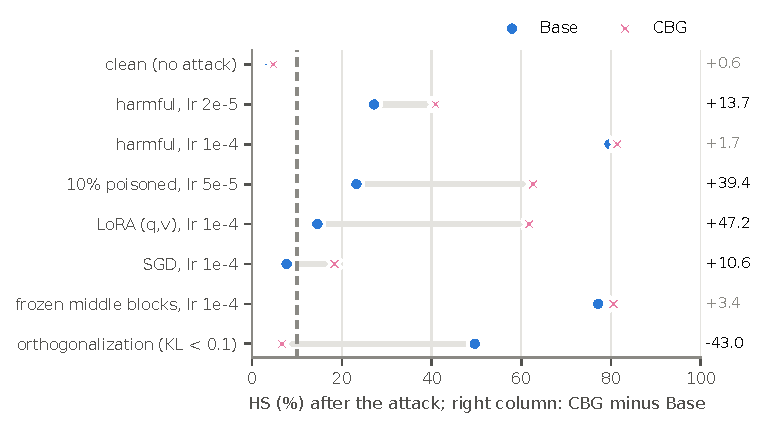
\includegraphics[width=\linewidth]{figures/fig_base_vs_cbg.pdf}
\caption{HS (\%) of Base and CBG after every attack in this paper, one run each. Right column: CBG minus Base. Dashed line: HS $=10\%$. CBG is more harmful than Base under every fine-tuning attack, by the largest margins under the weak ones (poisoned data, LoRA, SGD). Orthogonalization at KL $<0.1$ is the only attack under which it is safer (\cref{sec:orthogonal}).}
\label{fig:base_vs_cbg}
\end{figure}

\paragraph{SEAM's trap does not trigger self-destruction.}
SEAM's attack losses are 2.8--4.3 times Base's (\cref{tab:attack_loss}): its unlearning trap is active. Yet ZS after the attacks stays at 43.0--46.4, close to SEAM's clean 46.0, while HS reaches Base's level. The trap slows the fitting of the attack data, but it neither stops the model from becoming harmful nor collapses its utility.



\subsection{Full Learning-Rate Sweep}
\label{sec:exp_lr}

To match SEAM's main robustness experiment, we extend the harmful attack to its full learning-rate grid, adding $8\times10^{-5}$ and $2\times10^{-4}$ to the three rates of \cref{tab:main}. \Cref{tab:lr_sweep} compares CBG with Base and reports each attack's training loss; \cref{fig:lr_sweep} adds the other defenses. A defense that only slows fine-tuning would show a higher loss but the same final HS; one that self-destructs would show a sharp drop in ZS. The three rates of \cref{tab:main} are repeated from the same runs; the other two use the same protocol and input files. From $5\times10^{-5}$ on, HS saturates near 80 for both models while ZS declines slowly with the learning rate (to 45.0 for Base and 43.3 for CBG at $2\times10^{-4}$). Neither model self-destructs, and CBG's HS stays 1.5--5 points above Base's at every rate.

\begin{table*}[t]
\centering
\caption{Harmful attack learning-rate sweep (1{,}000 samples, 250 steps, seed 42). HS and ZS in \%; Loss is the mean attack training loss (padding tokens included).}
\label{tab:lr_sweep}
\resizebox{\textwidth}{!}{%
\begin{tabular}{lccccccccccccccc}
\toprule
& \multicolumn{3}{c}{$2\times10^{-5}$}
& \multicolumn{3}{c}{$5\times10^{-5}$}
& \multicolumn{3}{c}{$8\times10^{-5}$}
& \multicolumn{3}{c}{$1\times10^{-4}$}
& \multicolumn{3}{c}{$2\times10^{-4}$}\\
\cmidrule(lr){2-4}\cmidrule(lr){5-7}\cmidrule(lr){8-10}\cmidrule(lr){11-13}\cmidrule(lr){14-16}
Model & HS$\downarrow$ & ZS & Loss & HS$\downarrow$ & ZS & Loss & HS$\downarrow$ & ZS & Loss & HS$\downarrow$ & ZS & Loss & HS$\downarrow$ & ZS & Loss\\
\midrule
Base & 27.2 & 51.5 & 1.166 & 76.6 & 50.3 & 0.935 & 79.7 & 49.6 & 0.877 & 79.7 & 48.9 & 0.857 & 79.8 & 45.0 & 0.876\\
CBG & 40.9 & 46.1 & 1.301 & 81.7 & 46.1 & 1.033 & 81.3 & 45.9 & 0.947 & 81.4 & 45.7 & 0.920 & 81.4 & 43.3 & 0.925\\
\bottomrule
\end{tabular}}
\end{table*}

\begin{figure*}[t]
\centering
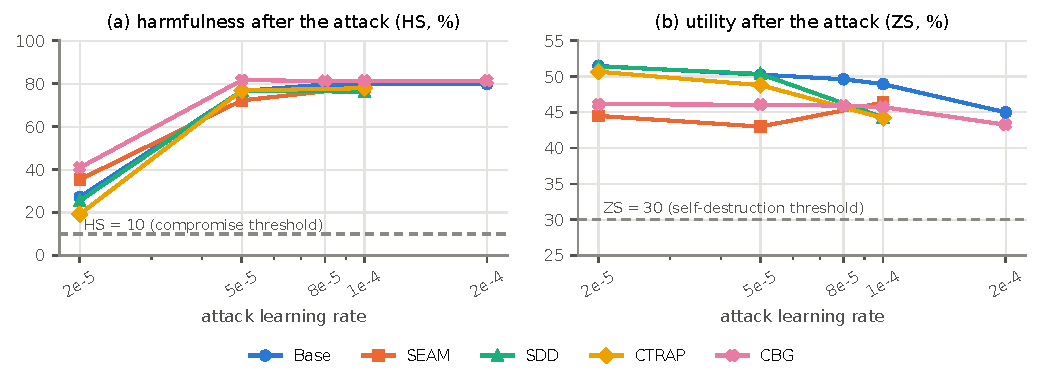
\includegraphics[width=\textwidth]{figures/fig_lr_sweep.pdf}
\caption{HS and ZS after harmful fine-tuning at each learning rate, one run each. SEAM, SDD and CTRAP were attacked only at the three rates of \cref{tab:main}. Dashed lines: the compromise threshold HS $=10\%$ and the self-destruction threshold ZS $=30\%$. No model approaches self-destruction.}
\label{fig:lr_sweep}
\end{figure*}



\subsection{Sensitivity to Decoding}
\label{sec:exp_decoding}

HS in the main comparison uses seeded sampling, as SEAM's evaluation script does. To check that conclusions do not depend on this choice, we re-measure HS with greedy decoding (\cref{tab:decoding}); the sampled columns repeat \cref{tab:main}, and the greedy runs repeat the same attacks. Greedy and sampled HS differ by at most 1.6 points, and CBG remains above Base after the attack under both, so the conclusions do not depend on the decoding.

\begin{table}[t]
\centering
\small
\caption{HS (\%) under greedy and sampled decoding, before and after the $1\times10^{-4}$ attack.}
\label{tab:decoding}
\begin{tabular}{lcccc}
\toprule
& \multicolumn{2}{c}{Pre-attack} & \multicolumn{2}{c}{After $1\times10^{-4}$}\\
\cmidrule(lr){2-3}\cmidrule(lr){4-5}
Model & Greedy & Sampled & Greedy & Sampled\\
\midrule
Base & 4.1 & 4.1 & 78.1 & 79.7\\
CBG  & 3.8 & 4.7 & 81.6 & 81.4\\
\bottomrule
\end{tabular}
\end{table}



\subsection{Attack Variants}
\label{sec:exp_variants}

We next vary the attack itself, keeping learning rates of $5\times10^{-5}$ and $1\times10^{-4}$:
\begin{itemize}
  \item \textbf{Data size:} 10{,}000 harmful samples instead of 1{,}000.
  \item \textbf{Parameter-efficient fine-tuning:} LoRA~\citep{hu2022lora} with rank 8, $\alpha=16$, on the query/value projections and on all linear modules.
  \item \textbf{Optimizer:} SGD instead of AdamW.
  \item \textbf{Long training at small learning rates:} up to 50K steps at $10^{-6}$ and $5\times10^{-6}$.
  \item \textbf{Frozen layers:} fine-tuning with the middle half of the decoder blocks (blocks 8--23 of 32) frozen.
\end{itemize}
For each variant, \cref{tab:variants} reports HS, ZS and whether the attacked model is compromised. So far three variants have been run, each otherwise following the protocol of \cref{sec:setting}: LoRA (q,v) (rank 8, $\alpha=16$), plain SGD (no momentum), and frozen middle blocks. The LoRA attack separates the two models sharply:
\begin{itemize}
  \item \textbf{Base} stays mostly safe: HS 14.5, with 12\% of responses above 0.5. 32\% of its responses are empty, and many of the others are refusals.
  \item \textbf{CBG} becomes harmful: HS 61.8, with 65\% of responses above 0.5 and no empty response, while ZS stays at 45.6.
  \item \textbf{Fitting does not explain it:} CBG's LoRA attack loss is higher than Base's (1.792 vs.\ 1.606), so CBG becomes more harmful despite fitting the attack data less well.
\end{itemize}
A low-capacity attack that barely affects the undefended model thus removes CBG's safety, consistent with the single benign-coupled safety direction of \cref{sec:barrier_analysis}.

The SGD attack shows the same pattern at a smaller scale:
\begin{itemize}
  \item \textbf{Base} is not compromised: HS 7.7, 4\% of responses above 0.5, attack loss 1.042.
  \item \textbf{CBG} is compromised: HS 18.3, 14\% of responses above 0.5, despite a higher attack loss (1.305).
  \item \textbf{Utility:} CBG's ZS falls from 47.4 to 43.5, mostly on HellaSwag (55.8 to 48.7). This is a partial loss of utility, not self-destruction.
\end{itemize}
With the middle blocks frozen, the attack succeeds on both models (HS 77.1 and 80.5), much as full fine-tuning does; the defended and attacked parameters are not confined to the middle of the network.
\todo{10K samples, LoRA on all linear modules and long training at small learning rates not run yet.}

\begin{table*}[t]
\centering
\small
\caption{Attack variants (HS / ZS in \%). Comp.: Yes if the attacked model is compromised (HS $>10\%$ and ZS $>30\%$), otherwise No.}
\label{tab:variants}
\begin{tabular}{lcccc}
\toprule
& \multicolumn{2}{c}{Base} & \multicolumn{2}{c}{CBG}\\
\cmidrule(lr){2-3}\cmidrule(lr){4-5}
Attack & HS / ZS & Comp. & HS / ZS & Comp.\\
\midrule
10K samples, $5\times10^{-5}$          & \tbd\ / \tbd & \tbd & \tbd\ / \tbd & \tbd\\
10K samples, $1\times10^{-4}$          & \tbd\ / \tbd & \tbd & \tbd\ / \tbd & \tbd\\
LoRA (q,v), $1\times10^{-4}$           & 14.5 / 50.9 & Yes & 61.8 / 45.6 & Yes\\
LoRA (all), $1\times10^{-4}$           & \tbd\ / \tbd & \tbd & \tbd\ / \tbd & \tbd\\
SGD, $1\times10^{-4}$                  & 7.7 / 51.7 & No & 18.3 / 43.5 & Yes\\
50K steps, $10^{-6}$                   & \tbd\ / \tbd & \tbd & \tbd\ / \tbd & \tbd\\
Frozen middle layers, $1\times10^{-4}$ & 77.1 / 50.6 & Yes & 80.5 / 45.0 & Yes\\
\bottomrule
\end{tabular}
\end{table*}



\subsection{Escape-Seeking Attacks}
\label{sec:adaptive}

An adaptive attacker who knows CBG can target low-collateral directions instead of following the plain harmful gradient. We evaluate four such attacks against CBG and Base (\cref{tab:adaptive}):
\begin{enumerate}
  \item \textbf{Utility-preserving:} adds $\lambda\,\mathrm{KL}(p_{\theta_0}\Vert p_\theta)$ on benign prompts to $\Lhfa$, with $\lambda\in\{0.01,0.05,0.1,0.2\}$ and $\theta_0$ the pre-attack defended model.
  \item \textbf{Projected:} removes from each attack gradient its component in the span of per-example benign gradients. This is the direction family that CBG penalizes as $\mu\to0$ (\cref{prop:degenerate}).
  \item \textbf{Reverse-CBG:} adds $-\beta'\log\etak$ to the attack loss, mirroring SEAM's trap reversal.
  \item \textbf{Renormalization:} a function-preserving rescaling of each SwiGLU block before fine-tuning (\cref{prop:reparam}).
\end{enumerate}
We also add Gaussian noise to the harmful gradient ($\sigma\in\{0.1,0.5,1\}$ relative to its RMS). Since the plain attack already compromises CBG (\cref{tab:main}), these attacks matter only once a configuration resists it. \todo{not run yet.}

\begin{table*}[t]
\centering
\small
\caption{Escape-seeking attacks at $5\times10^{-5}$ (HS / ZS in \%).}
\label{tab:adaptive}
\begin{tabular}{lcc}
\toprule
Attack & Base & CBG\\
\midrule
Utility-preserving ($\lambda=0.1$) & \tbd\ / \tbd & \tbd\ / \tbd\\
Projected                          & \tbd\ / \tbd & \tbd\ / \tbd\\
Reverse-CBG                        & -- & \tbd\ / \tbd\\
Renormalization                    & \tbd\ / \tbd & \tbd\ / \tbd\\
Gradient noise ($\sigma=0.5$)      & \tbd\ / \tbd & \tbd\ / \tbd\\
\bottomrule
\end{tabular}
\end{table*}



\subsection{Orthogonalization}
\label{sec:orthogonal}

We apply refusal-direction orthogonalization~\citep{arditi2024refusal} to Base and CBG. This edit is not a fine-tuning step and lies outside our theory, so the experiment tests transfer only.

\paragraph{Procedure.}
The attacker works on the evaluated model itself and never sees the test prompts.
\begin{itemize}
  \item \textbf{Candidate directions:} for every layer below $0.8L$, the difference between the mean residual-stream input at the last prompt token for 128 harmful prompts (attack set) and for 128 harmless prompts (Alpaca), with SEAM's template. Layer 0 is skipped, since at the last template token it holds only the token embedding and gives no direction.
  \item \textbf{Selection:} each direction is ablated at every layer and position, using 32 further prompts of each kind. We measure the refusal rate as a refusal-phrase match on 32 greedy tokens of the harmful prompts, and the KL divergence of the next-token distribution on the harmless prompts. Following \citet{arditi2024refusal}, the direction with the lowest refusal rate among those with KL $<0.1$ is chosen.
  \item \textbf{Edit:} the chosen direction is projected out of the embeddings and of every attention-output and MLP-down projection.
\end{itemize}
The edited model is evaluated like the \texttt{clean} case (\cref{sec:setting}). We report HS, the fraction of responses with score $>0.5$ (the attack success rate, ASR), and ZS.

\begin{table}[t]
\centering
\small
\caption{Refusal-direction orthogonalization (one run per model). Refusal: validation refusal rate (\%) before and after the edit. KL: harmless next-token KL of the chosen direction.}
\label{tab:orthogonal}
\resizebox{\linewidth}{!}{%
\begin{tabular}{lcccccc}
\toprule
Model & Layer & Refusal & KL & HS$\downarrow$ & ASR$\downarrow$ & ZS\\
\midrule
Base & 17 & 72 $\to$ 3 & 0.08 & 49.6 & 49 & 51.3\\
CBG  & 6  & 75 $\to$ 69 & 0.09 & 6.7 & 4 & 47.3\\
\bottomrule
\end{tabular}}
\end{table}

\begin{figure*}[t]
\centering
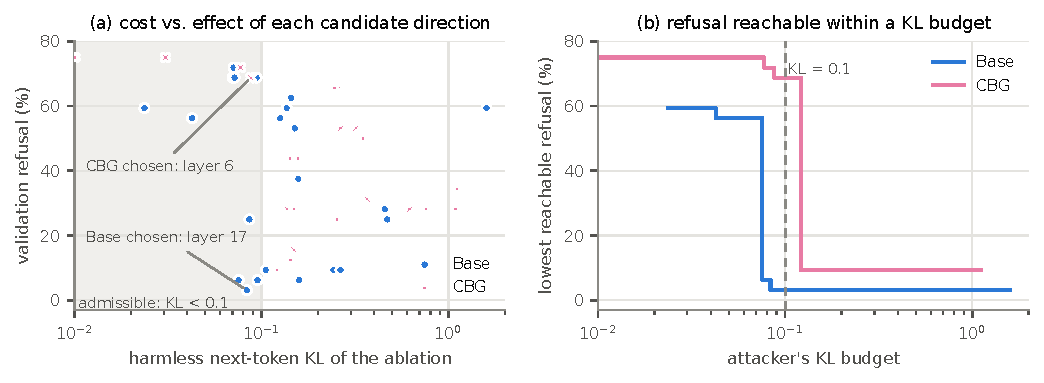
\includegraphics[width=\textwidth]{figures/fig_orthogonalization.pdf}
\caption{Refusal-direction candidates, one point per layer and model. (a) Validation refusal against the harmless next-token KL of ablating the direction; the shaded band is the admissible region of \citet{arditi2024refusal}. (b) The lowest refusal an attacker can reach within a KL budget. CBG moves the cheap refusal-removing directions just past KL $=0.1$.}
\label{fig:orthogonalization}
\end{figure*}

\paragraph{Results.}
\Cref{fig:orthogonalization} shows every candidate direction. On Base, the edit removes refusal at almost no benign cost: validation refusal falls from 72\% to 3\% (layer 17, KL 0.08), and HS rises from 4.1 to 49.6 while ZS stays at 51.3 (\cref{tab:orthogonal}). On CBG, no layer meets the KL constraint and also removes refusal:
\begin{itemize}
  \item \textbf{Within KL $<0.1$}, the best direction (layer 6) leaves 69\% refusal, and the edited model stays safe (HS 6.7, ASR 4\%).
  \item \textbf{Above it}, directions that do remove refusal exist: layers 16--17 leave 9--12\% refusal, but at KL 0.12--0.14. On Base, comparable directions cost 0.08--0.10.
\end{itemize}
CBG thus raises the benign cost of the cheapest refusal-removing edit, which is the effect the no-cheap-escape principle targets. The margin is small, however: an attacker who accepts a KL of 0.15 instead of 0.1 would likely succeed. The outcome rests on one direction-selection run with 32 validation prompts, and the KL threshold is a convention, not a property of the model. \todo{evaluate the edit at the best direction under KL $<0.15$, and repeat the selection with more prompts.}

% ----------------------------------------------------------------------------
\subsection{Geometry Analysis}
\label{sec:barrier_analysis}

\paragraph{Training dynamics.}
\Cref{tab:geometry} tracks the held-out geometry and the training losses of the final CBG run. They test whether $\etak$ falls through benign coupling, as intended, rather than through flattening, uniform inflation of benign gradients, or degradation of the model (rising $\Lbgn$).

\begin{table*}[t]
\centering
\small
\caption{Geometry and losses during the final CBG run. Geometry: held-out, mean over the 8 batches of $\mathcal D_{\mathrm{geo}}$ ($\mu=\tr K_{bb}/n$, $m=8$, $n=32$); erank: effective rank. Losses: training batches, mean over the 50 steps before the listed step (step 0: first step). $\mathcal L_{\mathrm{harm}}$ is the cross-entropy of the harmful responses at $\theta$ and at $\theta'=\theta-10^{-5}\operatorname{sign}(\nabla\mathcal L_{\mathrm{harm}})$, measured on the CBG steps.}
\label{tab:geometry}
\begin{tabular}{rcccccccccc}
\toprule
Step & $\log\etak$ & $\sigma_{1:k}$ & $\nu_{1:k}$ & $\tr K_{bb}$ & erank $K_{hh}$ & erank $K_{bb}$ & $\Laln$ & $\Lbgn$ & $\mathcal L_{\mathrm{harm}}(\theta)$ & $\mathcal L_{\mathrm{harm}}(\theta')$\\
\midrule
0   & $-0.024$ & 0.642 & 0.654 & 773.9 & 4.42 & 18.6 & 0.118 & 0.000 & 1.94 & 1.23\\
100 & $-0.189$ & 0.457 & 0.608 & 415.3 & 3.14 & 18.5 & 0.405 & 0.155 & 2.32 & 1.11\\
200 & $-0.829$ & 0.725 & 1.183 & 419.4 & 1.52 & 12.2 & 0.421 & 0.293 & 2.13 & 0.87\\
300 & $-1.625$ & 0.643 & 3.168 & 452.8 & 1.15 & 5.9 & 0.339 & 0.269 & 2.45 & 1.12\\
400 & $-1.397$ & 1.230 & 4.821 & 358.7 & 1.10 & 9.2 & 0.271 & 0.255 & 2.87 & 1.05\\
500 & $-1.534$ & 1.565 & 6.851 & 382.4 & 1.10 & 7.8 & 0.251 & 0.229 & 3.09 & 1.21\\
\bottomrule
\end{tabular}
\end{table*}

\begin{figure*}[t]
\centering
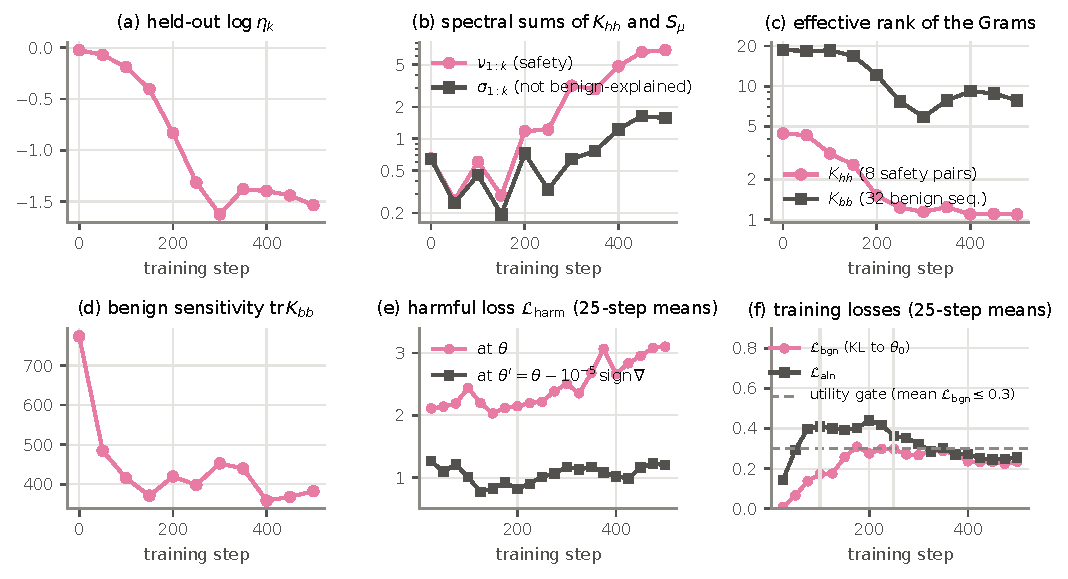
\includegraphics[width=\textwidth]{figures/fig_training_dynamics.pdf}
\caption{The final CBG run. (a--d) Held-out geometry on $\mathcal D_{\mathrm{geo}}$, every 50 steps: $\log\etak$, the spectral sums $\nu_{1:k}$ of $K_{hh}$ and $\sigma_{1:k}$ of $S_\mu$, the effective ranks of the two Grams, and the benign sensitivity $\tr K_{bb}$. (e) Harmful loss of the training pairs at $\theta$ and one sign step away. (f) Training losses and the utility gate. Means over 25 steps on the training batches in (e, f).}
\label{fig:geometry}
\end{figure*}

\Cref{tab:geometry} and \cref{fig:geometry} show four effects.
\begin{itemize}
  \item \textbf{$\etak$ falls through coupling.} $\etak$ falls from 0.977 to 0.223, not through flattening or benign inflation:
    \begin{itemize}
      \item the safety sensitivity $\nu_{1:k}$ grows 10.5-fold, while its part not explained by benign directions, $\sigma_{1:k}$, grows only 2.4-fold;
      \item the benign sensitivity $\tr K_{bb}$ halves;
      \item benign drift stays within the gate.
    \end{itemize}
    In this sense CBG does what it is designed to do: the safety-sensitive directions become increasingly aligned with benign ones.
  \item \textbf{Safety collapses onto one direction.} The effective rank of $K_{hh}$ falls from 4.4 to 1.1, and its top eigenvalue carries 96\% of the trace at step 500 (41\% at step 0). The safety gradients of the eight pairs collapse onto one direction.
  \item \textbf{Harmful behavior stays one sign step away.} The harmful loss rises at $\theta$ (1.94 to 3.09), yet one sign step of size $10^{-5}$ along the harmful gradient still brings it to about 1.2. The drop grows from 0.72 to 1.88 nats.
  \item \textbf{The barrier is local.} In the pilots, the held-out $\log\etak$ after 25 attack steps was $-0.11$ (pilot B, $-0.60$ before the attack) and $-0.39$ (C2, $-1.11$ before the attack), against $-0.05$ for Base (\cref{tab:selection}). The two-point term made the change more persistent but did not lower the validation HS.
\end{itemize}

\paragraph{Interpretation.}
Together with \cref{tab:main}, these observations suggest the following mechanism.
\begin{itemize}
  \item \textbf{What CBG produces:} a model whose safety behavior is concentrated in a single, strongly benign-coupled direction and is reachable by a short step from $\theta$.
  \item \textbf{Why benign coupling does not deter the attacker:} it raises the benign cost of moving along that direction, but the attack is not penalized for benign change, as long as ZS stays above the threshold.
  \item \textbf{Why poisoned data hurts most:} benign samples can push the model along the same direction. This is consistent with the largest gap to Base appearing under 10\% poisoning.
\end{itemize}
This is an interpretation of correlational evidence from one run. Attack checkpoints with geometry measurements are needed to test it.

\paragraph{Does geometry predict outcomes?}
Across the configurations of \cref{tab:selection}, larger decreases of $\log\etak$ did not come with lower attack HS. \todo{correlate the pre-attack $\etak$ with the ZS drop at matched HS increase across checkpoints and learning rates, and measure the escape ratio at attack checkpoints, which tests the path-bound assumption of \cref{prop:path}.}

% ----------------------------------------------------------------------------
\subsection{Ablations}
\label{sec:ablation}

Starting from the selected configuration, we change one component at a time and report held-out $\Delta\log\etak$, pre-attack ZS, and HS/ZS after the $5\times10^{-5}$ attack (\cref{tab:ablation}). The ablations are:
\begin{enumerate}
  \item $\log\etak$ versus raw $\rhohat$;
  \item $\Lam$ versus Euclidean damping;
  \item $k\in\{1,2,4,8\}$;
  \item sampled versus empirical Fisher;
  \item $n\in\{8,32,128\}$ at a fixed token budget;
  \item exact solve versus Rayleigh ascent with $K\in\{1,3,5\}$ iterations;
  \item exact Hessian--vector product versus finite differences, at several radii $r$ and in FP32 versus BF16;
  \item removing $\Laln$ or $\Lbgn$;
  \item detached versus differentiated $\mu$;
  \item one versus several sign draws, and the shared direction versus per-example perturbations;
  \item lazy period $1$ versus $4$;
  \item CBG versus CBG+UL versus UL alone ($\beta=0$).
\end{enumerate}
The last comparison isolates the contribution of the geometry term from that of the unlearning loss. Only the selected row has been run; the configurations of \cref{tab:selection} differ in several components at once and are therefore not listed here. \todo{not run yet.}

\begin{table*}[t]
\centering
\small
\caption{Ablations. Attack: $5\times10^{-5}$, HS / ZS in \%.}
\label{tab:ablation}
\begin{tabular}{lccc}
\toprule
Variant & $\Delta\log\etak$ & Pre ZS$\uparrow$ & Attack HS / ZS\\
\midrule
CBG (selected)              & $-1.51$ & 47.4 & 81.7 / 46.1\\
UL only ($\beta=0$)         & \tbd & \tbd & \tbd\ / \tbd\\
CBG+UL                      & \tbd & \tbd & \tbd\ / \tbd\\
Raw $\rhohat$               & \tbd & \tbd & \tbd\ / \tbd\\
Euclidean damping           & \tbd & \tbd & \tbd\ / \tbd\\
Empirical Fisher            & \tbd & \tbd & \tbd\ / \tbd\\
Detached $\mu$              & \tbd & \tbd & \tbd\ / \tbd\\
Without $\Lbgn$             & \tbd & \tbd & \tbd\ / \tbd\\
Lazy period 1               & \tbd & \tbd & \tbd\ / \tbd\\
\bottomrule
\end{tabular}
\end{table*}

% ----------------------------------------------------------------------------
\subsection{Overhead}
\label{sec:overhead}

\Cref{tab:overhead} reports the cost of the final CBG run on two H200 GPUs.
\begin{itemize}
  \item \textbf{Time:} a full CBG step, with the geometry evaluated at $\theta$ and $\theta'$, takes 48.3\,s on average. One geometry evaluation consists of a center pass of 1.2\,s, a Gram contraction of 8.0\,s, a direction pass of 6.5\,s and a curvature pass of 7.0\,s. A plain step takes 2.2\,s.
  \item \textbf{Total:} with a lazy period of 4, the mean is 13.8\,s per step and 2.4\,h for 500 steps, including the held-out geometry evaluations.
\end{itemize}
The baselines were trained on different hardware, so their times are not comparable and are omitted. \todo{measure the baselines on 2$\times$H200.}

\begin{table*}[t]
\centering
\small
\caption{Training cost on 2$\times$H200 (500 steps). Peak memory: the larger of the two GPUs, allocated by PyTorch.}
\label{tab:overhead}
\begin{tabular}{lccc}
\toprule
Method & Time / step (s) & Peak memory (GiB) & Total (h)\\
\midrule
SEAM   & \tbd & \tbd & \tbd\\
SDD    & \tbd & \tbd & \tbd\\
CTRAP  & \tbd & \tbd & \tbd\\
CBG    & 13.8 & 108.1 & 2.4\\
\bottomrule
\end{tabular}
\end{table*}




\section{Conclusion}
\label{sec:conclusion}

Self-destructive defenses make a chosen harmful adaptation costly, but an adaptive attacker can look for another route that removes safety at little benign cost. We proposed the no-cheap-escape principle, which makes the cheapest such route the defense target, and Collateral Barrier Geometry, which identifies the most collateral-efficient local directions out of safety and trains the model so that they incur benign damage. The broader takeaway is that a self-destructive defense should be judged by its weakest escape rather than by the attack it was trained against.

Empirically, the principle is not yet realized.
\begin{itemize}
  \item \textbf{What CBG achieves:} on Llama-2-7B-Chat it lowers the measured escape efficiency $\etak$ fourfold, through increased benign coupling as designed. At the conventional KL threshold it also blocks refusal-direction orthogonalization, though by a small margin.
  \item \textbf{What it does not achieve:} it does not prevent harmful fine-tuning. Under a shared protocol, neither do SEAM, SDD or CTRAP. CBG is even more vulnerable than the undefended model under poisoned fine-tuning and under a LoRA attack.
  \item \textbf{Why:} the learned geometry concentrates safety in a single benign-coupled direction and fades within the first steps of an attack.
\end{itemize}
Making a collateral barrier persist along real attack trajectories, and keeping it from making safety easier to remove, is the open problem these results point to.

\section*{Limitations}

CBG's guarantees are local: they concern a first-order quadratic model at the released parameters and imply nothing about long fine-tuning trajectories, non-local edits such as weight orthogonalization, or updates outside the admissible space $\U$. The geometry is defined by the sampled safety and benign data, so behavior those samples do not cover is unmeasured. It is also estimated from small minibatches, which makes the trained quantity $\etak$ a biased, damping-dependent estimate with a noisy gradient. The normalization in $\etak$ rules out uniform safety flattening and uniform benign inflation only, and invariance holds only for diagonal rescaling symmetries. Each CBG step needs several forward and backward passes and stores per-layer inputs and output gradients (\cref{app:impl}). Our evaluation covers one model, Llama-2-7B-Chat, and English safety data.
\begin{itemize}
  \item \textbf{Single runs:} every number comes from one defense run and one attack seed, and HS rests on 100 prompts.
  \item \textbf{Baselines:} SDD is a reimplementation, CTRAP was trained for 500 steps, and SEAM uses its released code, including an off-by-one loss mask.
  \item \textbf{Data:} the evaluation follows SEAM's protocol, which does not remove prompts shared between the defense, attack and test pools.
\end{itemize}

\bibliographystyle{acl_natbib}
\bibliography{sn-bibliography}

% =========================================================
% Appendix
% =========================================================
\appendix

\section{Theoretical Analysis of Collateral Barrier Geometry}
\label{app:cbg_theory}

Throughout, $\U\subseteq\R^p$ is a nonzero linear subspace, $\Gh,\Gb$ are symmetric positive semidefinite, and $Q_h(u)=u^\top\Gh u$, $Q_b(u)=u^\top\Gb u$. Every quadratic form satisfies $Q(-u)=Q(u)$; positive semidefiniteness gives $Q\ge0$ and $u^\top Gu=0\Leftrightarrow Gu=0$. We write
\begin{equation*}
\begin{gathered}
\Nb=\U\cap\ker\Gb,\qquad \Nh=\U\cap\ker\Gh,\\
\mathcal S=\U\cap\Nb^\perp .
\end{gathered}
\end{equation*}
Standard facts are cited; results without a citation are ours.

% ---------------------------------------------------------
\subsection{Exact Semidefinite Collateral Geometry}
\label{app:cbg_exact_geometry}

\begin{proposition}[Zero-collateral escape]
\label{prop:zero}
If $\Nb\not\subseteq\Nh$, then for every $\gamma>0$ there is $u_\gamma\in\U$ with $Q_h(u_\gamma)=\gamma^2$ and $Q_b(u_\gamma)=0$.
\end{proposition}
\begin{proof}
Take $v\in\Nb\setminus\Nh$ and $u_\gamma=\gamma v/\sqrt{Q_h(v)}$.
\end{proof}

Under $\Nb\subseteq\Nh$, every $u\in\U$ decomposes uniquely as $u=s+n$ with $s\in\mathcal S$ and $n\in\Nb$, and then $Q_b(u)=Q_b(s)$ and $Q_h(u)=Q_h(s)$; moreover $\Gb$ is positive definite on $\mathcal S$. With $P_{\mathcal S}$ an orthonormal basis of $\mathcal S$, let
\begin{equation*}
A=P_{\mathcal S}^\top\Gh P_{\mathcal S}\succeq0,\qquad B=P_{\mathcal S}^\top\Gb P_{\mathcal S}\succ0,
\end{equation*}
and define $\Resc=\lambda_{\max}(A,B)$ when $Q_h\not\equiv0$ on $\U$.

\begin{theorem}[Semidefinite local collateral barrier]
\label{thm:barrier}
Fix $\gamma>0$.
(i)~If $Q_h\equiv0$ on $\U$, then $\Resc=0$ and $\Barrier_\gamma=+\infty$.
(ii)~If $\Nb\not\subseteq\Nh$, then $\Resc=+\infty$ and $\Barrier_\gamma=0$.
(iii)~Otherwise $0<\Resc<\infty$ and $\Barrier_\gamma=\gamma^2/(2\Resc)$, attained by a scaled dominant generalized eigenvector.
\end{theorem}
\begin{proof}
(i)~The constraint is infeasible. (ii)~By \cref{prop:zero}. (iii)~Some $u\in\U$ has $Q_h(u)=Q_h(s)>0$, so $A\ne0$ and $\Resc>0$; finiteness follows from $B\succ0$. By the decomposition the problem reduces to $\mathcal S$. For feasible $v$,
\begin{equation*}
\gamma^2\le v^\top Av\le\Resc\,v^\top Bv,
\end{equation*}
so $\tfrac12v^\top Bv\ge\gamma^2/(2\Resc)$. If $Av^\star=\Resc Bv^\star$ and $t=\gamma/\sqrt{{v^\star}^\top Av^\star}$, then $tv^\star$ is feasible with cost $\gamma^2/(2\Resc)$.
\end{proof}

\begin{remark}[The $+\infty$ convention is the supremum]
Let $\Nb\not\subseteq\Nh$ and $Q_b\not\equiv0$ on $\U$, and pick $v\in\Nb\setminus\Nh$ and $w\in\U$ with $Q_b(w)>0$. Since $\Gb v=0$, $Q_b(v+\epsilon w)=\epsilon^2Q_b(w)$ while $Q_h(v+\epsilon w)\to Q_h(v)>0$, so the ratio over $\{Q_b>0\}$ is unbounded. The convention is needed only when $Q_b\equiv0$ on $\U$.
\end{remark}

The theorem is exact for the specified quadratic model. It does not assert that $Q_h(u)\ge\gamma^2$ is equivalent to a successful jailbreak.

% ---------------------------------------------------------
\subsection{Admissible Sets}
\label{app:admissible}

\begin{proposition}[Monotonicity in the admissible set]
\label{prop:monotone}
Let $\mathcal V\subseteq\U$ be a cone ($tu\in\mathcal V$ for all $t>0$, $u\in\mathcal V$), and define
\begin{equation*}
\Barrier_\gamma(\mathcal V)=\inf\bigl\{\tfrac12Q_b(u):u\in\mathcal V,\ Q_h(u)\ge\gamma^2\bigr\},
\end{equation*}
and $\Barrier^{(\mu)}_\gamma(\mathcal V)$ analogously. Then $\Barrier_\gamma(\mathcal V)\ge\Barrier_\gamma(\U)$ and $\Barrier^{(\mu)}_\gamma(\mathcal V)\ge\Barrier^{(\mu)}_\gamma(\U)$. In particular, the modeled barrier against rank-$r$ LoRA on matrices contained in $\U$ is at least the barrier over $\U$.
\end{proposition}
\begin{proof}
An infimum over a subset is at least the infimum over the set, and the rank-$\le r$ updates of a matrix form a cone.
\end{proof}

If $u\mapsto Tu$ is an injective linear parameterization with range $\U$, the undamped efficiency equals $\lambda_{\max}(T^\top\Gh T,T^\top\Gb T)$ whenever the second matrix is positive definite, and it does not depend on $T$. The damped efficiency does, unless the damping transforms with $T$ (\cref{prop:reparam}).

% ---------------------------------------------------------
\subsection{Damping, Reparameterization, and Finite Samples}
\label{app:damping}

Let $\Lambda\succ0$ on $\U$ and $\mu>0$, and define $\rhoreg$ and $\Barrier^{(\mu)}_\gamma$ as in \cref{eq:damped}.

\begin{proposition}[Damped barrier and sandwich]
\label{prop:damped}
(i)~If $Q_h\not\equiv0$ on $\U$, then $\Barrier^{(\mu)}_\gamma=\gamma^2/(2\rhoreg)$; otherwise $\rhoreg=0$ and $\Barrier^{(\mu)}_\gamma=+\infty$.
(ii)~$\rhoreg\le\Resc$ always, strictly if $0<\Resc<\infty$.
(iii)~If $\Nb\subseteq\Nh$ and $Q_h\not\equiv0$ on $\U$, let
\begin{equation*}
\kappa_\Lambda=\min_{s\in\mathcal S\setminus\{0\}}\frac{Q_b(s)}{s^\top\Lambda s}>0 .
\end{equation*}
Then
\begin{equation}
\begin{gathered}
\rhoreg\le\Resc\le\Bigl(1+\frac{\mu}{\kappa_\Lambda}\Bigr)\rhoreg,\\
\frac{\Barrier^{(\mu)}_\gamma}{1+\mu/\kappa_\Lambda}\le\Barrier_\gamma\le\Barrier^{(\mu)}_\gamma .
\end{gathered}
\label{eq:app_sandwich}
\end{equation}
(iv)~$\rhoreg$ is nonincreasing in $\mu$, and $\rhoreg\to\Resc$ as $\mu\downarrow0$, including when $\Resc=+\infty$.
\end{proposition}
\begin{proof}
(i)~$\Gb+\mu\Lambda$ is positive definite on $\U$; apply the argument of \cref{thm:barrier}(iii).
(ii)~If $Q_b(u)>0$ and $Q_h(u)>0$, then
\begin{equation*}
\frac{Q_h(u)}{Q_b(u)+\mu u^\top\Lambda u}<\frac{Q_h(u)}{Q_b(u)}\le\Resc .
\end{equation*}
If $Q_b(u)=0$ and $\Resc<\infty$, then $Q_h(u)=0$. For strictness, the damped maximizer has $Q_h>0$, hence $Q_b>0$, and its damped ratio lies strictly below its undamped ratio.
(iii)~For $u=s+n$ the undamped ratio equals $Q_h(s)/Q_b(s)$, and $s^\top\Lambda s\le Q_b(s)/\kappa_\Lambda$ gives
\begin{equation*}
\frac{Q_h(s)}{Q_b(s)+\mu s^\top\Lambda s}\ge\frac{Q_h(s)}{Q_b(s)\,(1+\mu/\kappa_\Lambda)} .
\end{equation*}
Taking suprema gives the upper bound on $\Resc$ in \cref{eq:app_sandwich}, and (i) gives the barrier form.
(iv)~Monotonicity holds pointwise in $u$. If $\Resc<\infty$, (iii) gives convergence. If $\Resc=\infty$, take $v\in\Nb\setminus\Nh$; then $\rhoreg\ge Q_h(v)/(\mu\,v^\top\Lambda v)\to\infty$.
\end{proof}

\begin{proposition}[Reparameterization]
\label{prop:reparam}
Let $\psi$ be a diffeomorphism of parameter space with $F_h\circ\psi=F_h$ and $F_b\circ\psi=F_b$, and let $D=D\psi(\theta)$.
(i)~$\Ch(\psi(\theta))D=\Ch(\theta)$ and $\Cb(\psi(\theta))D=\Cb(\theta)$, so $\Resc$ and $\Barrier_\gamma$ computed at $\psi(\theta)$ over $D\U$ equal those at $\theta$ over $\U$.
(ii)~The damped quantities are invariant if and only if $D^\top\Lambda_{\psi(\theta)}D=\Lam$ on $\U$. For a diagonal symmetry $\psi_c(\theta)=\diag(c)\theta$ with $c>0$ and a coordinate subspace $\U$, the metric $\Lam=\diag(\theta_i^{-2})$ satisfies this, whereas $\Lam=I$ does so only if $c=\mathbf 1$ on $\U$.
(iii)~If $f\circ\psi_c=f$ for a one-parameter group $\psi_c$, then
\begin{equation*}
\bigl\langle\nabla f(\theta),\,\partial_c\psi_c(\theta)|_{c=1}\bigr\rangle=0 ;
\end{equation*}
a damped objective that is not invariant generically has a nonzero derivative along the orbit, so gradient descent can lower it by a function-preserving move.
\end{proposition}
\begin{proof}
(i)~Differentiate $\Ft\circ\psi=\Ft$ by the chain rule and substitute $u'=Du$.
(ii)~The damping term becomes $\mu u^\top D^\top\Lambda_{\psi(\theta)}Du$. For $D=\diag(c)$ and $\Lambda_{\psi(\theta)}=\diag((c_i\theta_i)^{-2})$ this equals $\mu\sum_iu_i^2/\theta_i^2$.
(iii)~Differentiate $f(\psi_c(\theta))=f(\theta)$ at $c=1$.
\end{proof}
Diagonal symmetries of pre-norm transformers include: a normalization gain against the corresponding input columns of the following projection; an MLP up-projection row against the matching down-projection column (the gated activation is linear in the up-projection); matching query and key dimensions, with rotary pairs scaled equally; and value dimensions against the matching output-projection columns. General linear symmetries are not covered, and the floor $\xi>0$ makes invariance approximate for $|\theta_i|\lesssim\xi$. This mirrors the reparameterization critique of sharpness~\citep{dinh2017sharp} and its adaptive remedy~\citep{kwon2021asam}.

\begin{proposition}[Finite-sample degeneracy and small-damping limit]
\label{prop:degenerate}
Identify $\U$ with $\R^d$ by a coordinate selection, let $\Ch\in\R^{m\times d}$ and $\Cb\in\R^{n\times d}$ be the restricted weighted Jacobians, and write $\widetilde C=C\Lambda^{-1/2}$ for either of them.
(i)~$\Nb\subseteq\Nh$ if and only if $\row(\Ch)\subseteq\row(\Cb)$. Hence if $\operatorname{rank}[\Ch;\Cb]>\operatorname{rank}\Cb$, in particular if $m+n\le d$ and the $m+n$ rows are linearly independent, then $\Resc=+\infty$ and $\Barrier_\gamma=0$.
(ii)~Let $P_\perp$ be the orthogonal projector onto $\ker\widetilde C_b$. Then, for all $\mu>0$,
\begin{equation}
\begin{gathered}
\mu\,\rhoreg\ \ge\ \lambda_{\max}\bigl(\widetilde C_hP_\perp\widetilde C_h^\top\bigr),\\
\lim_{\mu\downarrow0}\mu\,\rhoreg=\lambda_{\max}\bigl(\widetilde C_hP_\perp\widetilde C_h^\top\bigr).
\end{gathered}
\label{eq:app_smallmu}
\end{equation}
\end{proposition}
\begin{proof}
(i)~$\ker(C^\top C)=\ker C$, and $\ker\Cb\subseteq\ker\Ch$ if and only if $\row\Ch\subseteq\row\Cb$.
(ii)~By \cref{prop:reduced},
\begin{equation*}
\rhoreg=\lambda_{\max}\bigl(\widetilde C_h(\widetilde C_b^\top\widetilde C_b+\mu I)^{-1}\widetilde C_h^\top\bigr).
\end{equation*}
If $\widetilde C_b^\top\widetilde C_b=\sum_i\sigma_i^2e_ie_i^\top$, then
\begin{equation*}
\begin{aligned}
\mu(\widetilde C_b^\top\widetilde C_b+\mu I)^{-1}&=\sum_{\sigma_i>0}\frac{\mu}{\sigma_i^2+\mu}\,e_ie_i^\top+P_\perp\\
&\succeq P_\perp ,
\end{aligned}
\end{equation*}
which is nondecreasing in $\mu$ and tends to $P_\perp$. The map $Y\mapsto\lambda_{\max}(XYX^\top)$ is monotone in the Loewner order and continuous.
\end{proof}

\begin{remark}[Relation to SEAM]
\label{rem:seam}
By \cref{eq:app_smallmu}, with small damping the finite-sample objective penalizes the largest energy of per-example safety-margin gradients outside the span of per-example benign gradients. SEAM's cosine loss~\citep{wang2026seam} drives one mean harmful gradient toward the negative of one mean benign gradient, i.e.\ into a one-dimensional benign span with a prescribed sign. CBG is a multi-direction, sign-agnostic analogue over every example in the batch: for $k=1$ and $\mu\downarrow0$,
\begin{equation*}
\eta_1\ \to\ \frac{\lambda_{\max}(\widetilde C_hP_\perp\widetilde C_h^\top)}{\lambda_{\max}(\widetilde C_h\widetilde C_h^\top)},
\end{equation*}
a generalized squared sine between the two spans. Moreover, the damped ratio of every $u\in\U$ is at most $\rhoreg$, including the restriction to $\U$ of the harmful gradient that SEAM targets.
\end{remark}

\begin{proposition}[Minibatch bias and consistency]
\label{prop:jensen}
Let $\Ghh$ and $\Gbh$ be independent, integrable random positive-semidefinite matrices with means $\bar{\mathcal G}_h$ and $\bar{\mathcal G}_b$, and let $f(A,B)=\lambda_{\max}(A,B+\mu\Lambda)$. Then
\begin{equation*}
\mathbb E\,f(\Ghh,\Gbh)\ \ge\ f(\bar{\mathcal G}_h,\bar{\mathcal G}_b).
\end{equation*}
If the minibatch metrics are averages of $m$ and $n$ i.i.d.\ terms, then $f(\Ghh,\Gbh)\to f(\bar{\mathcal G}_h,\bar{\mathcal G}_b)$ almost surely as $m,n\to\infty$.
\end{proposition}
\begin{proof}
For fixed $B$, $A\mapsto f$ is a pointwise maximum of linear functions, hence convex. For fixed $A\succeq0$, the map $B\mapsto(u^\top Au)/(u^\top(B+\mu\Lambda)u)$ is convex on the positive-definite cone, as a nonnegative multiple of the convex function $1/x$ composed with an affine map~\citep{boyd2004convex}, and so is its maximum over $u$. Jensen's inequality in $A$, conditionally on the independent $B$, and then in $B$ gives the bound. Consistency follows from the strong law of large numbers in finite dimension and continuity of $f$ for $\mu>0$; matrix Bernstein bounds give rates under bounded per-example gradients~\citep{tropp2012user}.
\end{proof}

\begin{proposition}[Sampled per-token Fisher]
\label{prop:mcfisher}
Fix $\theta$, a prompt $x$ and a reference $y$. Draw $\hat y_t\sim p_\theta(\cdot\mid x,y_{<t})$ independently over $t$, and let $s=\sum_t\nabla_\theta\log p_\theta(\hat y_t\mid x,y_{<t})$. Then $\mathbb E[ss^\top]=\sum_tF_t$, where $F_t$ is the Fisher information of $p_\theta(\cdot\mid x,y_{<t})$:
\begin{equation*}
F_t=\mathbb E_{v\sim p_\theta(\cdot\mid x,y_{<t})}\bigl[g_t(v)g_t(v)^\top\bigr],
\end{equation*}
with $g_t(v)=\nabla_\theta\log p_\theta(v\mid x,y_{<t})$. Moreover,
\begin{equation*}
\begin{aligned}
&\textstyle\sum_t D_{\mathrm{KL}}\bigl(p_\theta(\cdot\mid x,y_{<t})\,\Vert\,p_{\theta+u}(\cdot\mid x,y_{<t})\bigr)\\
&\quad=\tfrac12u^\top\Bigl(\textstyle\sum_tF_t\Bigr)u+o(\|u\|_2^2).
\end{aligned}
\end{equation*}
\end{proposition}
\begin{proof}
The score has zero mean under the model, so the cross terms $\mathbb E[s_ts_{t'}^\top]=\mathbb E[s_t]\mathbb E[s_{t'}]^\top$ vanish for $t\ne t'$ by independence. The KL expansion is the standard Fisher identity~\citep{amari1998natural,martens2020new}.
\end{proof}

% ---------------------------------------------------------
\subsection{Normalized Collateral Efficiency}
\label{app:eta}

\begin{proposition}[Properties of $\etak$]
\label{prop:eta}
Let $\Bmu=\Gbh+\mu\Lam$ and $1\le k\le\operatorname{rank}(\Ghh|_\U)$.
(i)~$\rho_j\le\nu_j/\mu$ for every $j$, hence $0<\etak\le1$.
(ii)~$\etak$ is unchanged under $\Ch\mapsto t\Ch$, under $(\Cb,\mu)\mapsto(t\Cb,t^2\mu)$, and under the diagonal symmetries of \cref{prop:reparam} with $\xi=0$.
(iii)~For $k=1$, let
\begin{equation*}
\Barrier^{(\mu,0)}_\gamma=\inf\bigl\{\tfrac12\mu\,u^\top\Lam u:u\in\U,\ Q_h(u)\ge\gamma^2\bigr\}
\end{equation*}
be the cost of the cheapest escape when benign collateral is ignored. Then $\Barrier^{(\mu)}_\gamma=\Barrier^{(\mu,0)}_\gamma/\eta_1$.
\end{proposition}
\begin{proof}
(i)~By the Courant--Fischer characterization for definite pencils~\citep{parlett1998symmetric},
\begin{equation*}
\rho_j=\max_{\dim\mathcal V=j}\ \min_{u\in\mathcal V\setminus\{0\}}\frac{u^\top\Ghh u}{u^\top\Bmu u},
\end{equation*}
and $\Bmu\succeq\mu\Lam$ together with $u^\top\Ghh u\ge0$ gives $\rho_j\le\nu_j/\mu$. Positivity holds because $\rho_1>0$ when $\Ghh|_\U\ne0$.
(ii)~In the first case numerator and denominator both scale by $t^2$. In the second, $\Bmu\mapsto t^2\Bmu$, so $\rho_j\mapsto\rho_j/t^2$ and $\mu\rho_j$ is unchanged. The third follows from \cref{prop:reparam}.
(iii)~Apply \cref{prop:damped}(i) with $\Gbh$ replaced by $0$: $\Barrier^{(\mu,0)}_\gamma=\gamma^2\mu/(2\nu_1)$, while $\Barrier^{(\mu)}_\gamma=\gamma^2/(2\rho_1)$.
\end{proof}

\begin{remark}[Detached versus differentiated $\mu$]
\label{rem:mu}
Property (ii) concerns values. The value of $\etak$ is invariant under $(\Cb,\mu)\mapsto(t\Cb,t^2\mu)$ only because $\mu=\kappa_\mu\tr(K_{bb})/n$ moves with the benign Gram. With $\mu$ detached, the gradient ignores this, and uniformly inflating benign sensitivity lowers $\etak$ (\cref{tab:numerical}). Since $\partial\Smu/\partial\mu=K_{hb}(\mu I_n+K_{bb})^{-2}K_{hb}^\top$,
\begin{equation*}
c_\mu:=\frac{\partial\log\etak}{\partial\mu}=\frac{\sum_{j\le k}\|z_j\|^2}{\sigma_{1:k}}\ \ge0,
\end{equation*}
and differentiating $\mu$ adds $(\kappa_\mu/n)\,c_\mu E_b$ to $\partial\log\etak/\partial K$, the $E_b$ term of \cref{eq:G}. Its coefficient is nonnegative, so it raises the objective when $\tr K_{bb}$ grows and penalizes benign inflation. In terms of the damped escapes, $c_\mu=1/\mu-\sum_j\rho_j\|D_\theta^{-1}u_j\|^2/\sum_j\rho_j$, which is nonnegative because $\mu\|D_\theta^{-1}u_j\|^2\le Q_b(u_j)+\mu\|D_\theta^{-1}u_j\|^2=1$.
\end{remark}

% ---------------------------------------------------------
\subsection{Exact Reduced Solve}
\label{app:reduced}

\begin{proposition}[Reduced system]
\label{prop:reduced}
Let $\widetilde C=CD_\theta=[\Cth;\Ctb]$, $K=\widetilde C\widetilde C^\top$ and $\Smu$ as in \cref{eq:reduced}.
(i)~$\Cth\Pmu\Cth^\top=\Smu$. Hence the nonzero generalized eigenvalues of $(\Ch^\top\Ch,\ \Cb^\top\Cb+\mu\Lam)$ on $\U$ are $\sigma_j/\mu$, where $\sigma_j$ runs over the positive eigenvalues of $\Smu$ with multiplicities, and those of $(\Ch^\top\Ch,\Lam)$ are the positive eigenvalues $\nu_j$ of $K_{hh}$.
(ii)~If $\Smu\phi=\sigma\phi$ with $\sigma>0$ and $\|\phi\|=1$, let $z=(\mu I_n+K_{bb})^{-1}K_{hb}^\top\phi$, $\psi=(\phi;-z)$ and $u=D_\theta\widetilde C^\top\psi/\sqrt{\mu\sigma}$. Then
\begin{equation*}
\begin{gathered}
\Ch^\top\Ch u=\tfrac{\sigma}{\mu}\bigl(\Cb^\top\Cb+\mu\Lam\bigr)u,\\
Q_b(u)+\mu\,u^\top\Lam u=1,\\
\Ch u=\sqrt{\sigma/\mu}\,\phi,\qquad \Cb u=\sqrt{\mu/\sigma}\,z .
\end{gathered}
\end{equation*}
(iii)~If $K_{hh}\phi'=\nu\phi'$ with $\nu>0$ and $\|\phi'\|=1$, then $v=\Lam^{-1}\Ch^\top\phi'/\sqrt\nu$ satisfies $\Ch^\top\Ch v=\nu\Lam v$ and $v^\top\Lam v=1$.
\end{proposition}
\begin{proof}
Work in relative coordinates $\delta=D_\theta^{-1}u$, where the pencil becomes $(\Cth^\top\Cth,B)$ with $B=\Ctb^\top\Ctb+\mu I=\mu\Pmu^{-1}$. (i)~The nonzero eigenvalues of $B^{-1}\Cth^\top\Cth$ equal those of $\Cth B^{-1}\Cth^\top=\mu^{-1}\Cth\Pmu\Cth^\top$~\citep{horn2012matrix}. The push-through identity
\begin{equation*}
(\mu I+\Ctb^\top\Ctb)^{-1}\Ctb^\top=\Ctb^\top(\mu I_n+K_{bb})^{-1}
\end{equation*}
gives $\Pmu=I-\Ctb^\top(\mu I_n+K_{bb})^{-1}\Ctb$ and hence $\Cth\Pmu\Cth^\top=\Smu$~\citep{golub2013matrix}. (ii)~By the same identity, $\delta:=D_\theta^{-1}u=\Pmu\Cth^\top\phi/\sqrt{\mu\sigma}$. Then $\Cth\delta=\Smu\phi/\sqrt{\mu\sigma}=\sqrt{\sigma/\mu}\,\phi$; $\Ctb\Pmu=\mu(\mu I_n+K_{bb})^{-1}\Ctb$ gives $\Ctb\delta=\sqrt{\mu/\sigma}\,z$; $B\delta=\mu\Cth^\top\phi/\sqrt{\mu\sigma}$, so $\Cth^\top\Cth\delta=\sqrt{\sigma/\mu}\,\Cth^\top\phi=(\sigma/\mu)B\delta$; and $\delta^\top B\delta=\phi^\top\Smu\phi/\sigma=1$. Returning to $u=D_\theta\delta$ gives the claims, since $\Ch u=\Cth\delta$, $\Cb u=\Ctb\delta$ and $u^\top\Lam u=\|\delta\|^2$. (iii)~is (ii) with $\Ctb=0$ and $\mu=1$.
\end{proof}

% ---------------------------------------------------------
\subsection{Gradient and Its Estimation}
\label{app:outer}

\paragraph{Assumptions.} $F_h,F_b$ are $C^4$ near $\theta$; samples, sampled targets and $W_h,W_b$ are fixed within a step; $\U$ is fixed; and $\xi>0$, so that $\Lam$ is smooth.

\begin{proposition}[Gram pull-back]
\label{prop:gram}
Let $f$ be differentiable at $K(\theta)=C(\theta)\Lam^{-1}C(\theta)^\top$, with symmetric gradient $G$, i.e.\ $df=\tr(G\,dK)$. Then
\begin{equation*}
\begin{aligned}
\nabla_\theta f\bigl(K(\theta)\bigr)={}&2\textstyle\sum_eH_{\Ft_e}w_e\\
&+2\,\theta\odot\operatorname{diag}(C^\top GC),
\end{aligned}
\end{equation*}
with $w_e=\Lam^{-1}C^\top G\mathbf 1_e$. Moreover $\operatorname{diag}(C^\top GC)=\Lam\sum_ec_e\odot w_e$ and $\|\Lam^{1/2}w_e\|^2=(GKG)_{ee}$.
\end{proposition}
\begin{proof}
Since $dc_e=H_{\Ft_e}d\theta$ and $d(\theta_i^2+\xi^2)=2\theta_i\,d\theta_i$,
\begin{equation*}
\begin{aligned}
dK_{ee'}={}&c_e^\top\Lam^{-1}H_{\Ft_{e'}}d\theta+(H_{\Ft_e}d\theta)^\top\Lam^{-1}c_{e'}\\
&+2\textstyle\sum_ic_{e,i}c_{e',i}\theta_i\,d\theta_i .
\end{aligned}
\end{equation*}
Summing against the symmetric $G$ and using the symmetry of each Hessian,
\begin{equation*}
\begin{aligned}
\tr(G\,dK)={}&2\textstyle\sum_{e}\bigl(H_{\Ft_e}\sum_{e'}G_{ee'}\Lam^{-1}c_{e'}\bigr)^\top d\theta\\
&+2\textstyle\sum_i\theta_i[C^\top GC]_{ii}\,d\theta_i ,
\end{aligned}
\end{equation*}
and $\sum_{e'}G_{ee'}\Lam^{-1}c_{e'}=w_e$. For the last two claims, $[C^\top GC]_{ii}=\sum_ec_{e,i}[\Lam w_e]_i$ and $\Lam^{1/2}w_e=\widetilde C^\top G\mathbf 1_e$.
\end{proof}

\begin{proposition}[Gradient of $\log\etak$]
\label{prop:gradient}
Let $\mu=\kappa_\mu\tr(K_{bb})/n$, and let $\phi_j,z_j,\psi_j$ and $\phi'_j,\psi'_j$ be as in \cref{eq:escape,eq:G}. If $\sigma_k>\sigma_{k+1}$ and $\nu_k>\nu_{k+1}$, then $\log\etak$ is differentiable in $K$ with gradient $G$ of \cref{eq:G}. With $\mu$ held fixed, the gradient is \cref{eq:G} without the $E_b$ term. Without the gap conditions, $\sigma_{1:k}$ and $\nu_{1:k}$ are locally Lipschitz in $K$, and the same expressions, built from any orthonormal basis of the top-$k$ eigenspaces, are Clarke subgradients.
\end{proposition}
\begin{proof}
By Ky Fan's principle, $\sigma_{1:k}=\max_{Y^\top Y=I_k}\tr(Y^\top\Smu Y)$; at a gap its differential is $\tr(\Phi_k^\top d\Smu\,\Phi_k)$ with $\Phi_k=[\phi_1,\dots,\phi_k]$~\citep{kato1995perturbation,magnus1985differentiating}. With $R=(\mu I_n+K_{bb})^{-1}$ and $Z=RK_{hb}^\top\Phi_k$,
\begin{equation*}
\begin{aligned}
d\Smu={}&dK_{hh}-dK_{hb}RK_{hb}^\top-K_{hb}R\,dK_{hb}^\top\\
&+K_{hb}R\,(dK_{bb}+d\mu\,I_n)\,RK_{hb}^\top,
\end{aligned}
\end{equation*}
so $\tr(\Phi_k^\top d\Smu\,\Phi_k)=\tr(\Psi_k\Psi_k^\top dK)+\|Z\|_F^2\,d\mu$ with $\Psi_k=[\Phi_k;-Z]$. Since $d\mu=(\kappa_\mu/n)\tr(E_b\,dK)$, this is $\tr\bigl([\Psi_k\Psi_k^\top+(\kappa_\mu/n)\|Z\|_F^2E_b]\,dK\bigr)$. Likewise $d\nu_{1:k}=\tr(\Psi'_k\Psi_k'^\top dK)$, and $d\log\etak=d\sigma_{1:k}/\sigma_{1:k}-d\nu_{1:k}/\nu_{1:k}$. Without gaps, each spectral sum is a maximum of smooth functions over a compact set, so it is locally Lipschitz and the gradients at maximizers generate its Clarke subdifferential~\citep[Sec.~2.8]{clarke1983optimization}; see also \citet{overton1993optimality}. Stochastic subgradient methods converge for such functions~\citep{davis2020stochastic}.
\end{proof}

\begin{proposition}[Curvature estimators]
\label{prop:randomized}
(i)~\emph{Shared direction.} If $a,b\in\R^{m+n}$ are random with $\mathbb E[ab^\top]=G$, $\Omega=a^\top\Ft$ and $w=\Lam^{-1}C^\top b$, then $\mathbb E[2H_\Omega w]=2\sum_eH_{\Ft_e}w_e$. The eigen-sign pair $a=V|\Gamma|^{1/2}s$, $b=V\operatorname{sgn}(\Gamma)|\Gamma|^{1/2}s$ with $G=V\Gamma V^\top$ and Rademacher $s$ satisfies $\mathbb E[ab^\top]=G$, and $\|\Lam^{1/2}w\|^2=b^\top Kb$.
(ii)~\emph{Per-example directions.} For radii $\varepsilon_e>0$,
\begin{equation*}
\begin{aligned}
&\textstyle\sum_e\frac{1}{\varepsilon_e}\bigl(\nabla\Ft_e(\theta+\varepsilon_ew_e)-\nabla\Ft_e(\theta-\varepsilon_ew_e)\bigr)\\
&\qquad=2\textstyle\sum_eH_{\Ft_e}w_e+\mathcal O\bigl(\max_e\varepsilon_e^2\bigr).
\end{aligned}
\end{equation*}
(iii)~For any fixed $\Omega$ and $w$,
\begin{equation}
\begin{aligned}
&\Bigl\|\tfrac{1}{\varepsilon}\bigl(\nabla\Omega(\theta+\varepsilon w)-\nabla\Omega(\theta-\varepsilon w)\bigr)-2H_\Omega w\Bigr\|\\
&\qquad\le\frac{\varepsilon^2}{3}\sup_{|\tau|\le\varepsilon}\bigl\|\nabla^4\Omega(\theta+\tau w)[w,w,w]\bigr\| .
\end{aligned}
\label{eq:app_fd}
\end{equation}
\end{proposition}
\begin{proof}
(i)~$H_\Omega w=\sum_{e,e'}a_eb_{e'}H_{\Ft_e}\Lam^{-1}c_{e'}$; taking expectations and using $\sum_{e'}G_{ee'}\Lam^{-1}c_{e'}=w_e$ gives the claim. For the eigen-sign pair, $\mathbb E[ab^\top]=V|\Gamma|^{1/2}\,\mathbb E[ss^\top]\operatorname{sgn}(\Gamma)|\Gamma|^{1/2}V^\top=G$, and $\Lam^{1/2}w=\widetilde C^\top b$. (ii) and (iii) are the centered-difference Taylor remainder in integral form~\citep{nocedal2006numerical}: even-order terms cancel, and the two third-order remainders each contribute at most $\tfrac{\varepsilon^3}{6}\sup\|\nabla^4\Omega[w,w,w]\|$ before division by $\varepsilon$, applied per example in (ii).
\end{proof}
The shared direction applies the Rademacher device of Hutchinson's trace estimator~\citep{hutchinson1989stochastic} to a sum of Hessian--vector products with different directions. It is unbiased up to $\mathcal O(\varepsilon^2)$ but has sign-draw variance (\cref{tab:numerical}); several draws can be averaged at two passes each. The per-example form has no sign variance, because examples do not interact in the forward pass and each can be evaluated at its own perturbation; with $\varepsilon_e=r\sqrt{\dim\U/(GKG)_{ee}}$, every example is perturbed to the same relative radius $r$. The Hessian--vector products could also be computed exactly by reverse-over-reverse differentiation~\citep{pearlmutter1994fast}, but that requires double-backward support in fused attention kernels, which the two-pass difference avoids.

\paragraph{Computing $d_\Lambda$.}
By \cref{prop:gram}, $\operatorname{diag}(C^\top GC)=\sum_ec_e\odot\bigl(\sum_{e'}G_{ee'}c_{e'}\bigr)$ in terms of the per-example gradients $c_e$. It is accumulated layer by layer in the chunked pass over the stored layer inputs and output gradients that also forms $w$ (\cref{app:impl}), so it requires no additional forward or backward pass.

\paragraph{Precision.}
In bf16 the relative spacing of a weight is $2^{-8}$~\citep{kalamkar2019study}, so coordinates of $\varepsilon w$ smaller than about $2^{-8}|\theta_i|$ are rounded away and the difference in \cref{eq:app_fd} becomes rounding noise (\cref{app:numerical}). Two roundings matter: storing $\theta\pm\varepsilon w$, and rounding inside each matrix multiplication (bf16 autocast rounds weights and activations to $2^{-8}$ relative, TF32 to about $2^{-11}$). Applying the shared perturbation to fp32 master weights removes the first. The per-example form applies $x_e(\theta\pm\varepsilon_ew_e)^\top=x_e\theta^\top\pm\varepsilon_e\,x_ew_e^\top$ as an additive branch, which also keeps the perturbation out of the weights. Neither removes the second, so $r$ must lie above the compute resolution and is set by comparing against an exact Hessian--vector product on a small model. The classical optimum for centered differences scales as the cube root of the working precision~\citep{nocedal2006numerical}.

\begin{proposition}[Finite-radius objective]
\label{prop:finite}
For fixed $u$ define
\begin{equation*}
a_\varepsilon=\frac{\|\Ft_h(\theta+\varepsilon u)-\Ft_h(\theta-\varepsilon u)\|^2}{4\varepsilon^2},
\end{equation*}
$b_\varepsilon$ analogously with $\Ft_b$ plus $\mu u^\top\Lam u$, and $R_\varepsilon=a_\varepsilon/b_\varepsilon$. Then $\nabla_\theta R_\varepsilon(\theta;u^\star)=\nabla_\theta\rhoreg+\mathcal O(\varepsilon^2)$ at an exact simple maximizer $u^\star$.
\end{proposition}
\begin{proof}
Write $\Delta_\varepsilon F=\Ft_h(\theta+\varepsilon u)-\Ft_h(\theta-\varepsilon u)$ and $\Delta_\varepsilon C=\Ch(\theta+\varepsilon u)-\Ch(\theta-\varepsilon u)$. Then $\Delta_\varepsilon F=2\varepsilon\Ch u+\mathcal O(\varepsilon^3)$ and $\Delta_\varepsilon C=2\varepsilon\,\partial\Ch[u]+\mathcal O(\varepsilon^3)$, so
\begin{equation*}
\begin{aligned}
\nabla a_\varepsilon&=\tfrac{1}{2\varepsilon^2}(\Delta_\varepsilon C)^\top\Delta_\varepsilon F\\
&=2\,\partial\Ch[u]^\top\Ch u+\mathcal O(\varepsilon^2)=\nabla a+\mathcal O(\varepsilon^2),
\end{aligned}
\end{equation*}
and likewise for $b_\varepsilon$. The envelope identity at $u^\star$ completes the proof.
\end{proof}
The gradient of $R_\varepsilon$ is exact for the finite-radius objective, which includes curvature within radius $\varepsilon$; it is an optional variant costing two extra forward passes.

% ---------------------------------------------------------
\subsection{From Local Geometry to Paths}
\label{app:path}

\begin{proposition}[Path-integrated barrier]
\label{prop:path}
Let $\theta:[0,1]\to\R^p$ be piecewise $C^1$ with $\dot\theta(t)\in\U$, and suppose the metrics along the path satisfy $Q_h^{\theta(t)}(v)\le\bar\rho\,Q_b^{\theta(t)}(v)$ for all $v\in\U$ and $t$. Then
\begin{equation*}
\begin{aligned}
&\bigl\|\Ft_h(\theta(1))-\Ft_h(\theta(0))\bigr\|_2\\
&\qquad\le\ \sqrt{\bar\rho}\int_0^1\Bigl\|\tfrac{d}{dt}\Ft_b(\theta(t))\Bigr\|_2\,dt .
\end{aligned}
\end{equation*}
If instead the damped ratio is bounded by $\bar\rho_\mu$, the right-hand side becomes
\begin{equation*}
\sqrt{\bar\rho_\mu}\Bigl(\int_0^1\bigl\|\tfrac{d}{dt}\Ft_b\bigr\|\,dt+\sqrt\mu\int_0^1\bigl\|\Lambda_{\theta(t)}^{1/2}\dot\theta\bigr\|\,dt\Bigr).
\end{equation*}
\end{proposition}
\begin{proof}
We have
\begin{equation*}
\begin{aligned}
\bigl\|\Ft_h(\theta(1))-\Ft_h(\theta(0))\bigr\|&=\Bigl\|\int_0^1\Ch\dot\theta\,dt\Bigr\|\\
&\le\int_0^1\sqrt{Q_h(\dot\theta)}\,dt\\
&\le\sqrt{\bar\rho}\int_0^1\sqrt{Q_b(\dot\theta)}\,dt,
\end{aligned}
\end{equation*}
and $\sqrt{Q_b(\dot\theta)}=\|\tfrac{d}{dt}\Ft_b(\theta(t))\|$. For the damped case use $\sqrt{x+y}\le\sqrt x+\sqrt y$.
\end{proof}
Any path that moves the safety margins by $\Delta$ must therefore move the benign outputs along a curve of length at least $\Delta/\sqrt{\bar\rho}$, provided the ratio bound holds along the path. This is an assumption, not a consequence of training. In our runs, most of the trained decrease of $\log\etak$ disappears within the first 25 steps of a real attack (\cref{sec:barrier_analysis}), so the assumption should not be expected to hold along such paths. The bound also explains why an amplification term that increases the margin displacement an attack must achieve, such as SEAM's unlearning loss, increases the required benign motion linearly.

% ---------------------------------------------------------
\subsection{Scope}
\label{app:scope}

\Cref{thm:barrier} and \cref{prop:damped,prop:eta,prop:path} concern specified quadratic models or paths along which a ratio bound holds. The trained quantity is the minibatch, damped, normalized $\etak$, differentiated through the Gram with a centered-difference or exact Hessian--vector curvature term. None of these results implies robustness to arbitrary harmful fine-tuning, jailbreak resistance, or capability destruction under non-local edits such as weight orthogonalization; those are empirical questions.

% =========================================================
\section{Implementation Details}
\label{app:impl}

\Cref{alg:cbg} lists one defense step; this appendix gives the layer-level details.

\paragraph{Stored tensors.}
The center pass stores, for every linear layer $Z=XW^\top$ in $\U$, the inputs $X$ and the output gradients $\Delta$ of the backward pass of $\mathbf 1^\top\Ft$ (\cref{alg:cbg}). Everything else in the step is formed from these tensors, so the graph is not retained and no second backward pass is run. By direct count they take about 5\,MB per token in bf16 for Llama-2-7B (about 40\,GB at 8{,}192 tokens) and can be offloaded to host memory layer by layer.

\paragraph{Per-example Gram accumulation.}
Let $X_e$ ($T_e\times d_{\mathrm{in}}$) and $\Delta_e$ ($T_e\times d_{\mathrm{out}}$) be the stored tensors on the tokens of example $e$. Because examples do not interact in the forward pass, the block of the per-example gradient $c_e$ belonging to this layer is $\Delta_e^\top X_e$; a safety example sums its two sequences. Inner products in the $\Lam^{-1}$ metric are
\begin{equation*}
K_{ee'}\mathrel{+}=\bigl\langle(\theta\odot\theta+\xi^2)\odot\Delta_e^\top X_e,\;\Delta_{e'}^\top X_{e'}\bigr\rangle ,
\end{equation*}
accumulated in float64. Per-example gradients are formed in chunks of output rows, so only part of one layer is held at a time. Holding all of them for a $14336\times4096$ matrix and $m+n=40$ examples would take about 4.7\,GB in bf16 (9.4\,GB in fp32) by direct count. When $\Lam^{-1}$ is replaced by the identity on a layer, the Gram can be formed without materializing per-example gradients~\citep{li2022large}.

\paragraph{Forming $w$ and $d_\Lambda$.}
After the eigensolve, one more chunked pass over the stored tensors re-forms the per-example gradients and computes, layer by layer, $w=\Lam^{-1}\odot\sum_eb_e\,\Delta_e^\top X_e$ and the diagonal $\sum_ec_e\odot\sum_{e'}G_{ee'}c_{e'}$ that gives $d_\Lambda$ (\cref{prop:gram}). The direction $w$ alone would need only one weighted matrix product per layer; $d_\Lambda$ is what requires the per-example form.

\paragraph{Per-example variant.}
Each linear layer computes $x_e\theta^\top\pm\varepsilon_e\,x_ew_e^\top$ on the tokens of example $e$, with $w_e=\Lam^{-1}C^\top G\mathbf 1_e$ and $\varepsilon_e=r\sqrt{\dim\U/(GKG)_{ee}}$. The $w_e$ of a layer are rebuilt chunk by chunk from the stored tensors in the forward pass and again in the backward pass, where the branch contributes to the input gradient; the scalarization of pass $\sigma$ is $\sum_e\sigma\beta\Ft_e/\varepsilon_e$.

\paragraph{Randomness.}
The sampled targets $\hat y$, dropout masks (disabled by default), sign draws and minibatches are shared between the center pass and both perturbed passes.

\paragraph{Cost (pass-count estimate, not a measurement).}
Let $G_{\mathrm{p}}$ be one forward and backward pass on 4{,}096 tokens. With $m=8$ safety pairs of at most 256 tokens per response and $n=32$ benign sequences of at most 128 tokens, a joint pass costs about $2G_{\mathrm{p}}$. Forming all per-example gradients costs about as much as one weight-gradient computation, roughly a third of a joint pass. One step with the shared direction then costs about $2G_{\mathrm{p}}$ for the center pass, $0.8G_{\mathrm{p}}$ for the Gram, a negligible eigensolve, $0.8G_{\mathrm{p}}$ for $w$ and $d_\Lambda$, $4G_{\mathrm{p}}$ for the two perturbed passes, and $0.3G_{\mathrm{p}}$ for the reference forward of $\Lbgn$: about $8G_{\mathrm{p}}$. SEAM's Algorithm~1 evaluates five to six gradients per step on batches of 8 examples~\citep{wang2026seam}; its token count per batch is not reported, so the ratio depends on it. The per-example variant adds the branch products and the rebuilding of $w_e$ to both perturbed passes, for about $14G_{\mathrm{p}}$ per step. Measured time and memory are reported in \cref{sec:overhead}.

% =========================================================
\section{Hyperparameters}
\label{app:hparams}

\Cref{tab:hparams} lists the settings of the final CBG run, selected on the validation protocol of \cref{sec:exp_selection} before any test attack. The attack configuration and the baseline settings are given in \cref{sec:setting}.

\begin{table}[h]
\centering
\small
\caption{CBG hyperparameters.}
\label{tab:hparams}
\begin{tabular}{@{}p{0.40\linewidth}p{0.52\linewidth}@{}}
\toprule
Setting & Value\\
\midrule
Admissible space $\U$ & all linear-layer weights in the transformer blocks\\
Safety pairs / step $m$ & 8 ($\le256$ tokens per sequence)\\
Benign sequences / step $n$ & 32 ($\le256$ tokens)\\
Spectral modes $k$ & 4\\
Damping scale $\mu$ & $\kappa_\mu\tr(K_{bb})/n$, differentiated\\
Curvature term & exact Hessian--vector product (TF32), shared eigen-sign direction, one draw\\
Loss weights $\alpha,\beta$ & $1$, $0.1$\\
Damping $\kappa_\mu$, floor $\xi$ & $1$, $10^{-3}$\\
Perturbation radius $r$ & not used by the exact product; $1.1\times10^{-7}$ in the finite-difference check\\
Two-point geometry & $\theta$ and $\theta-10^{-5}\operatorname{sign}(\nabla\mathcal L_{\mathrm{harm}})$, equal weights\\
Geometry gradient & per-tensor balance to $\|\nabla(\Laln+\alpha\Lbgn)\|$; clip at $3\times$ the median of the last 16\\
Lazy geometry & period 4, gradient reused on intermediate steps\\
Optimizer, lr, schedule, steps & AdamW, $2\times10^{-5}$, cosine with 10\% warmup, 500\\
Weight decay, gradient clipping & none, none\\
Utility gate & mean $\Lbgn$ of the last 20 steps $\le0.3$ at steps 100 and 250\\
\bottomrule
\end{tabular}
\end{table}

% =========================================================
\section{Attack Training Losses}
\label{app:attack_loss}

\Cref{tab:attack_loss} lists the mean training loss of every fine-tuning run of \cref{tab:main} and the loss of its first step. Losses include padding tokens (\cref{sec:setting}), which affects their absolute values; every model is trained on the same texts.

\begin{table}[h]
\centering
\small
\caption{Attack training loss, mean over 250 steps (first step in parentheses), same runs as \cref{tab:main}.}
\label{tab:attack_loss}
\resizebox{\linewidth}{!}{%
\begin{tabular}{lccccc}
\toprule
Model & h2e-5 & h5e-5 & h1e-4 & benign & mixed10\\
\midrule
Base & 1.166 (13.80) & 0.935 (13.80) & 0.857 (13.80) & 1.014 (9.89) & 0.895 (9.09)\\
SEAM & 5.004 (124.37) & 3.129 (124.37) & 2.386 (124.37) & 3.905 (53.58) & 2.675 (116.15)\\
SDD & 1.158 (13.71) & 0.930 (13.71) & 0.863 (13.71) & 1.006 (9.79) & 0.887 (9.00)\\
CTRAP & 1.053 (10.41) & 0.863 (10.41) & 0.815 (10.41) & 0.891 (6.98) & 0.822 (6.45)\\
CBG & 1.301 (11.74) & 1.033 (11.74) & 0.920 (11.74) & 1.074 (7.81) & 0.957 (8.48)\\
\bottomrule
\end{tabular}}
\end{table}

\Cref{fig:attack_loss} shows the loss curves at $10^{-4}$. SEAM's trap appears as a first-step loss near 124 that takes about 30 steps to reach the level of the other models. After that, all five curves coincide, so the trap delays fitting but does not prevent it. The per-scenario results of \cref{tab:main} are plotted in \cref{fig:main_comparison}.

\begin{figure}[h]
\centering
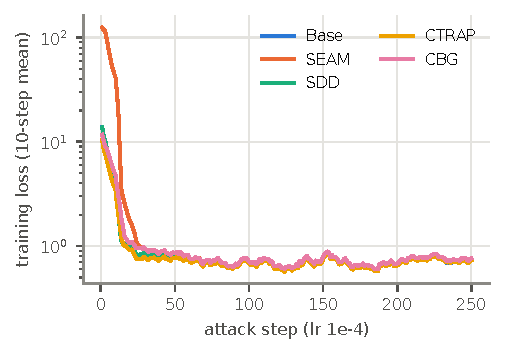
\includegraphics[width=0.85\linewidth]{figures/fig_attack_loss.pdf}
\caption{Attack training loss at learning rate $10^{-4}$ (10-step running mean, log scale), same runs as \cref{tab:main}.}
\label{fig:attack_loss}
\end{figure}

\begin{figure*}[h]
\centering
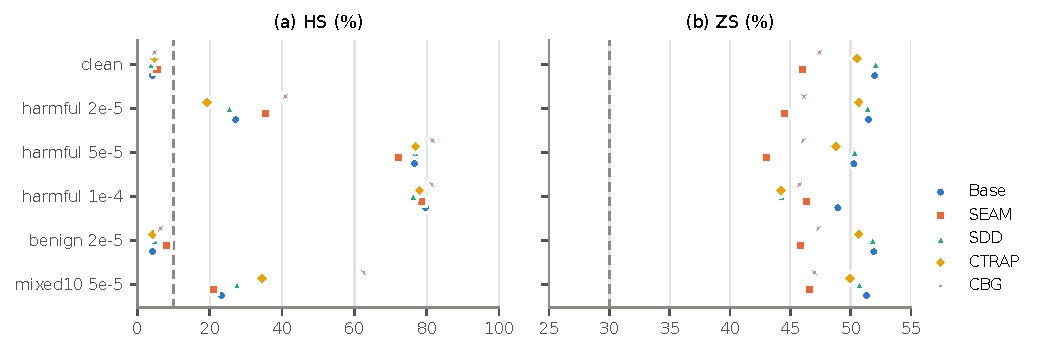
\includegraphics[width=\textwidth]{figures/fig_main_comparison.pdf}
\caption{The main comparison of \cref{tab:main} as a dot plot. Dashed lines: HS $=10\%$ and ZS $=30\%$.}
\label{fig:main_comparison}
\end{figure*}

% =========================================================
\section{Numerical Verification on a Synthetic Model}
\label{app:numerical}

We verified the identities and estimators used above in float64 on two small synthetic models with exact derivatives: a 60-parameter model with an RMS-normalized hidden layer and a normalization gain, which has exact function-preserving rescaling symmetries, and, for the rows marked $\dagger$, a 30-parameter analytic model with closed-form gradients and Hessians ($m=4$, $n=8$, $k=2$). \Cref{tab:numerical} lists the checks. They confirm the algebra; they say nothing about LLM behavior.

\begin{table*}[t]
\centering
\small
\caption{Synthetic checks of the theory (float64).}
\label{tab:numerical}
\begin{tabular}{@{}p{0.22\linewidth}p{0.72\linewidth}@{}}
\toprule
Result & Observation\\
\midrule
\Cref{thm:barrier}(iii) & constrained minimum matches $\gamma^2/(2\Resc)$ to $4\times10^{-12}$ relative (20 random pencils)\\
\Cref{prop:degenerate} & minibatch $\Gbh$ has rank 8 of 60; $\mu\rhoreg$ converges to $\lambda_{\max}(\widetilde C_hP_\perp\widetilde C_h^\top)$ as $\mu\to0$\\
\Cref{prop:damped}(iii) & sandwich holds on 50 random pencils\\
\Cref{prop:reduced} & top-3 eigenvalues and eigenvector agree with the full pencil to machine precision\\
\Cref{prop:reduced}(ii)$^\dagger$ & escape formulas (eigenvector, normalization, both displacements) hold to $1.4\times10^{-15}$\\
\Cref{prop:gram,prop:gradient}$^\dagger$ & Gram-gradient formula matches central differences of $\log\etak$ to $1.6\times10^{-9}$ ($\mu$ differentiated) and $1.5\times10^{-9}$ ($\mu$ held fixed); the alternative forms of $d_\Lambda$ and $\|\Lam^{1/2}w_e\|^2$ agree to $5\times10^{-16}$\\
\Cref{rem:mu}$^\dagger$ & $c_\mu$ matches $\partial\log\etak/\partial\mu$ to $4\times10^{-9}$; fivefold benign inflation leaves $\log\etak$ unchanged ($2\times10^{-16}$) but changes it by $0.41$ with $\mu$ held fixed\\
\Cref{prop:randomized}$^\dagger$ & expectation over all $2^{12}$ sign draws matches the curvature term to $3\times10^{-15}$; a single draw has $200\%$ mean relative error with the eigen-sign pair and $279\%$ with a plain Rademacher pair; the shared and per-example differences are second order (error ratio $4.00$ per halving)\\
\Cref{prop:finite} & gradient error is second order in $\varepsilon$\\
\Cref{prop:reparam} & a function-preserving rescaling changes Euclidean-damped $\rhoreg$ by $+44\%$; $\Lam$-damped $\rhoreg$ and $\eta_1$ unchanged\\
\Cref{prop:jensen} & minibatch mean exceeds the population value by $\approx18\times$, $5\times$, $2\times$ at $m=n=4,16,64$\\
\Cref{prop:mcfisher} & exact expectation equals the token-summed Fisher; KL ratio $0.99997$\\
\Cref{prop:path} & bound holds on a curved path\\
Precision & with bf16-rounded weights the centered difference has $190\%$, $35\%$, $6\%$ error at relative radii $10^{-4},10^{-3},10^{-2}$ (under $0.3\%$ unrounded)\\
\bottomrule
\end{tabular}
\end{table*}

\end{document}